\documentclass[]{article}

\usepackage[paperheight=18cm,paperwidth=14cm,textwidth=12cm]{geometry}
\usepackage[skip=20pt plus1pt, indent=40pt]{parskip}

\usepackage{hyperref}

\usepackage{graphicx}
\graphicspath{ {./images/} }
\usepackage{float}

\usepackage{amsmath}
\usepackage{amsfonts}
\usepackage{amssymb}

\def\mathcolor#1#{\@mathcolor{#1}}
\def\@mathcolor#1#2#3{%
  \protect\leavevmode
  \begingroup
    \color#1{#2}#3%
  \endgroup
}
\usepackage[dvipsnames]{xcolor}
\usepackage{sectsty}
\definecolor{bittersweet}{rgb}{1.0, 0.44, 0.37}
\definecolor{grey}{rgb}{0.25, 0.25, 0.28}
\definecolor{black}{rgb}{0, 0, 0}
\subsubsectionfont{\color{black}}
\subsubsectionfont{\color{grey}}
\sectionfont{\color{bittersweet}}

\usepackage[T1]{fontenc}
\renewcommand\familydefault{\sfdefault} 

\usepackage{bm}

\newcommand{\ev}{\mathbb{E}[X]}
\renewcommand{\ev}[1]{\mathbb{E}\left[#1\right]}
\newcommand*{\diff}{\mathop{}\!\mathrm{d}}

\newcommand{\definizione}{\paragraph{Definizione:}}
\newcommand{\formula}{\paragraph{Formula generica:}}

\newcommand{\highlight}[1]{\colorbox{yellow}{$\displaystyle #1$}}

\begin{document}
    \tableofcontents
    \newpage 
    \section{Introduzione}
    In probabilità quello che facciamo noi è quello di supporre che le nostre distribuzioni siano \textbf{note}, in statistica facciamo il contrario, ossia dire qualcosa (anche detto \textit{fare dell'inferenza}) su \textbf{parametri sconosciuti}. \\
    Dato che i parametri sono sconosciuti il massimo che possiamo fare è quello di ottenere \textit{una stima} dei parametri \textit{incogniti}. \\[2ex]
    Questi sono chiamati \textbf{stimatori puntuali} e sono indicati con il simbolo $\boldsymbol{\hat{\theta}}$ (in questo caso stiamo parlando di uno stimatore del parametro incognito $\boldsymbol{\theta}$) \\[2ex]
    Esisono anche gli \textit{stimatori non puntuali}, noti come \textbf{intervalli di confidenza}, ossia un intervallo di valori in cui può essere contenuto il \textit{dato incognito}.
    \begin{figure}[H]
        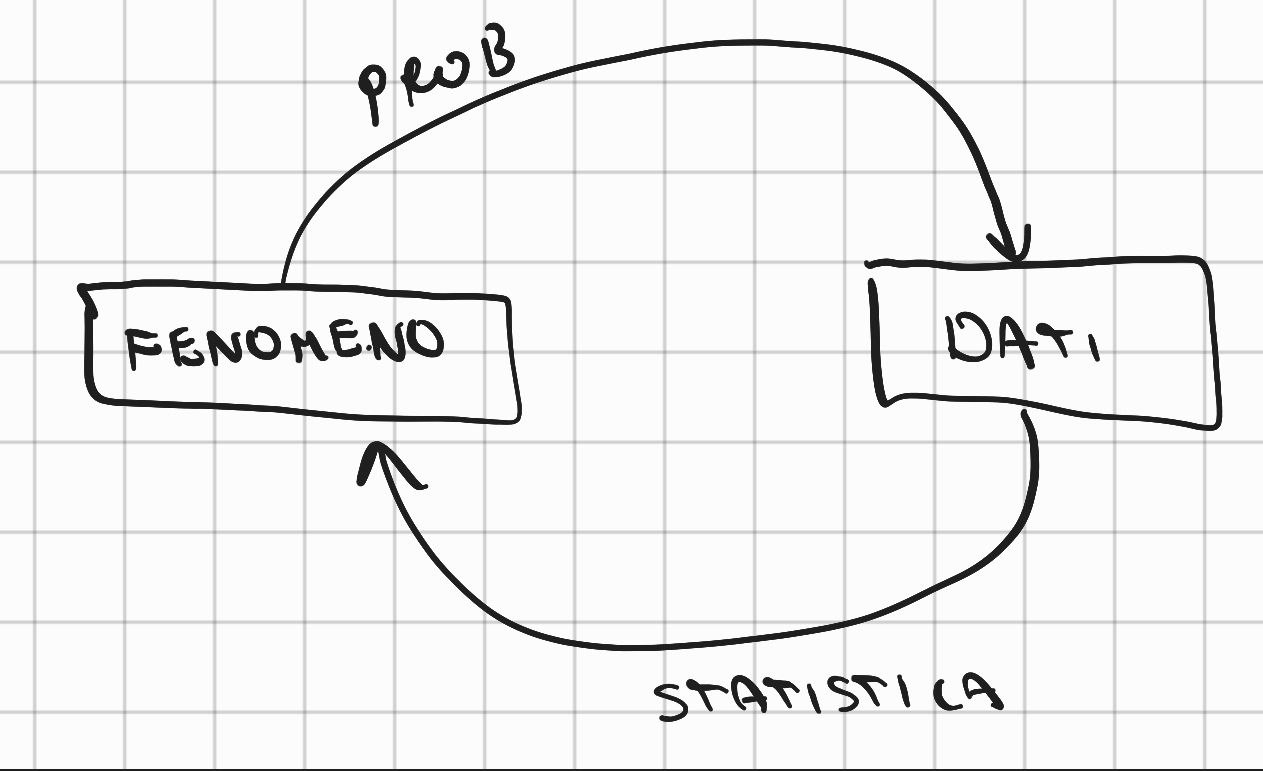
\includegraphics[width=\textwidth]{images/boh_15.jpg}
    \end{figure}
    \paragraph{Esempio} $\hat{\theta}? \quad \text{Altezza della popolazione}$ \\[2ex]
    \begin{minipage}{0.49\textwidth}
        $X_1 = 1.7$ \\
        $X_2 = 1.82$ \\
        $X_3 = 1.73$
    \end{minipage}
    \begin{minipage}{0.49\textwidth}
        $X_4 = 1.7$ \\
        $X_5 = 1.8$ \\
    \end{minipage}
    \paragraph{Possibile soluzione}: 
    \[ \hat{\theta_a} = \frac{1}{n} \sum_{4}^{5} x_i = \frac{1.7 + 1.82 + 1.73 + 1.7 + 1.8}{5} = \frac{8.75}{5} = 1.75 \]
    \[ \hat{\theta_b} = \frac{min(x_i) + \max(x_i)}{2} = \frac{3.52}{2} = 1.76 \]
    \[ \hat{\theta_c} = \frac{1}{3} \sum_{2}^{4} x_i = \frac{1}{3} (1.8 + 1.73 + 1.7) = \frac{5.23}{3} = 1.743 \]
    \centerline{Scartiamo il più \textit{piccolo} e il \textit{massimo}, calcolando poi la \textbf{media} dei rimanenti}
    \section{MLE}
    \definizione Stima a Massima Verosomiglianza (Maximum Likelihood Estimation) \\
    Questa classe di stimatori sono molto usati in statistica, servono per comparare molteplici modelli per \textit{determinare} quello che si adatta di più ai dati. \\
    Ad esempio la stima di massima verosomiglianza $\hat{\theta}$ è definita come il valore di $\theta$ che rende massima $\boldsymbol{f(x_1, x_2, \ldots, x_n \rvert \theta)} \rightarrow$ anche detta \textit{funziona di likelihood} \\[2ex]
    \textbf{Likelihood}: avendo dei dati quale è la probabilità che un certo modello descriva al meglio la natura dei nostri dati
    \[ \hat{\theta} = argmax L(\theta) = argmax[f(X_1 \ldots X_n / \theta )] \]
    \paragraph{Stima parametrica}(Point) Parametric Estimation \\ \\
    \underline{Ipotesi}:
    - Esiste un parametro $\theta$ incognito e $n$ dati a disposizione $\{X_1, X_2, X_n\}$ \\
    \textbf{Legge di probabilità} che descrive il fenomeno che ha generato i dati
    \formula Bayes
    \[ P(\theta / X_1 \ldots X_n) = \frac{P(X_1 \ldots X_n / \theta) P(\theta)}{P(X_1 \ldots X_n)} \]
    \centerline{Verosomiglianza (likelihood)}
    \subsection{MLE di una Bernoulliana}
    Vengono realizzate \textit{n} prove indipendenti con probabilità $p$ di successo
    \begin{equation*}
        X_i =
        \begin{cases}
            1 & \text{se la prova i-esima ha successo} \\
            0 & \text{altrimenti}
        \end{cases}
    \end{equation*}
    La distribuzione dell $X_i$ è la seguente:
    \[ P(X_i = k) = p^k (1-p)^{1-k}, \qquad k \in \{0,1\} \]
    La likelihood (ossia la \textit{funzione di massa congiunta}) è:
    \begin{equation*}
        \begin{split}
            f(x_1, x_2, \ldots, x_n \rvert p) &:= P(X_1 = x_1, X_2 = x_2, \ldots X_n = x_n \rvert p) \\
            &= p^{x1}(1-p)^{1-x1} \ldots p^{x_n}(1-p)^{1-x_n} \\
            &= p^{\sum_{i}^{} x_1}(1-p)^{n- \sum_{i}^{} x_1} \qquad x_1 = 0,1 \qquad i = 1, \ldots, n
        \end{split}
    \end{equation*}
    Derivando rispetto a $p$ possiamo ottenere un'espressione per la stima $\boldsymbol{\hat{p}}$:
    \[ \boldsymbol{\hat{p} = \frac{1}{n} \sum_{i = 1}^{n} x_i} \]
    \subsection{MLE di una Poisson}
    La funzione di \textit{likelihood} è data da:
    \begin{equation*}
        \begin{split}
            f(x_1, x_2 \ldots x_n / \lambda) &= \frac{\lambda^{x_1} e^{-y}}{x_1!} \ldots \frac{\lambda^{x_n} e^{-\lambda}}{x_n!} \\
            &= \frac{\lambda^{\sum_{i}^{} x_i} e^{-\lambda}}{x_1 ! \ldots x_n !} \\
        \end{split}
    \end{equation*}
    Derivando possiamo ottenere un'espressione per la stima $\hat{\lambda}$:
    \[ \hat{\lambda} = \frac{1}{n} \sum_{i = 1}^{n} x_i \]
    La stessa formula può essere applicata al campione $X_1, X_2, \ldots, X_n$:
    \[ P\{X_i = 1\} = 1 - P\{X_i = 0\} \]
    \paragraph{Esempio} Numero di incidenti stradali in 10 giornate senza pioggia \\
    Dataset: \{ 4 0 6 5 2 1 2 0 4 3 \} \\
    Si vuole stimare per quell'anno la frazione di giornate senza pioggia con \textit{2 incidenti o meno}
    \[ \overline{X} = \frac{1}{10} \sum_{i = 1}^{10} x_i = \boldsymbol{2.7} \]
    (capire sto risultato) Cosi otteniamo che la media della poissoniana è 2.7, la stima desiderata è data da:
    \[ (1+2.7+ (2.7)^2 /2 ) e^{-2.7} \approx 0.4936 \]
    \subsection{MLE distribuzione Uniforme}
    Per la MLE delle uniformi dobbiamo trovare i valori di limite \textit{inferiore} e \textit{superiore} che massimizzano la probabilità di ottenere i dati osservati.
    \begin{equation*}
        f(X_1, \ldots X_n \rvert \theta) =
        \begin{cases}
            \frac{1}{\theta} & 0 < x_1 < \theta \\
            0 & \text{altrimenti}
        \end{cases}
    \end{equation*}
    La formula per la stima di $\theta$:
    \[ \hat{\theta} = \max \{ X_1, \ldots, X_n \} \]
    $$ \hat{\theta}_{\frac{\text{MLE}}{2}} = \textit{media} $$
    \subsection{MLE distribuzione Normale } 
    \definizione La distribuzione normale ha media $\mu$ e dev. st. $\sigma$ \textbf{incognite} \\
    La densità congiunta (la likelihood) è data da:
    \[ f(x_1, x_2, \ldots, x_n \rvert \mu, \sigma) = \prod_{i= 1}^{n} \frac{1}{\sqrt{2 \mu \sigma}} \exp \left \{ - \frac{(x_1-\mu)^2}{2 \sigma^2} \right \} \]
    La log-likelihood è data da:
    \[ \log f(x_1, x_2, \ldots, x_n \rvert \mu, \sigma) = - \frac{n}{2} \log(2\pi) - n \log \sigma - \frac{1}{2\sigma^2} \sum_{i = 1}^{n} (x_i - \mu)^2 \]
    La risoluzione ci porta alle seguenti formule per le stime:
    \[ \hat{\mu} = \frac{1}{n} \sum_{i = 1}^{n} x_i \]
    \[ \hat{\sigma} = \sqrt{\frac{1}{n} \sum_{i = 1}^{n}(x_i - \hat{\mu})^2 } \]
    \section{Teorema del limite centrale}
    \definizione Questo teorema afferma che la somma di un numero elevato di \textbf{var. aleatorie indipendenti} tende ad avere una distribuzione approssimativamente normale.\\
    Quindi un campione (insieme di var. aleatorie da $X_1, X_2\ldots, X_n$) può essere trasformato in una Normale Standard:
    \[ \frac{X_1 + X_2 + \ldots + X_n - n\mu}{\sigma \sqrt{n}} \]
    \section{Intervalli di confidenza}
    \begin{figure}[H]
        \caption{Rappresentazione grafica}
        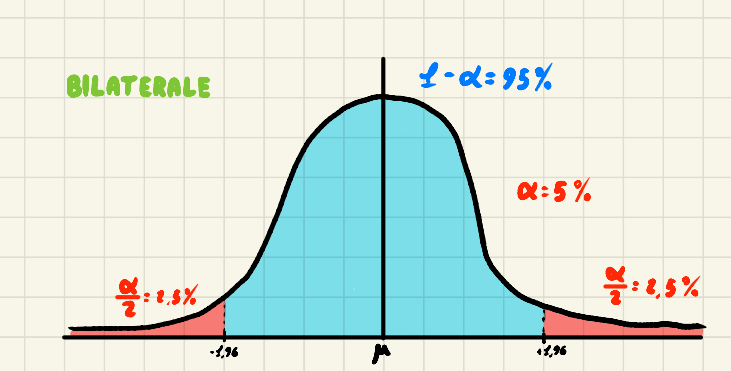
\includegraphics[width=\textwidth]{images/boh_16.png}
    \end{figure}
    \subsection{Distribuzione normale}
    \subsubsection{$\mu$ incognita e varianza  $\sigma^2$ nota}
    \definizione Sia $\boldsymbol{X_1, X_2, \ldots, X_n}$ un campione di una popolazione normale con $\mu$ \textit{incognita} e varianza $\sigma^2$ \textit{nota}:
    \[ \frac{\overline{X} - \mu}{\sigma / \sqrt{n}} \sim \mathcal{N}(0,1) \]
    Intervallo di confidenza per la media:
    \[ P \left( \overline{X} - 1.96 \frac{\sigma}{\sqrt{n}} < \mu < \overline{X} + 1.96 \frac{\sigma}{\sqrt{n}}\right) = 1-\alpha \]
    Il 95\% circa delle volte $\mu$ starà a una distanza non superiore a 1.96 $\sigma / \sqrt{n}$ dalla
    media aritmetica dei dati. Se osserviamo il campione, e registriamo che $\boldsymbol{\overline{X} = \overline{x}}$, allora possiamo dire che "con il 95\% di confidenza"
    \[ \left( \overline{x} - 1.96 \frac{\sigma}{\sqrt{n}}, \overline{x} + 1.96 \frac{\sigma}{\sqrt{n}} \right) \]
    \centerline{Questo intervallo è detto \textit{intervallo di confidenza} ad un livello del 95\%}
    \paragraph{intervallo destro:}
    $$ (\overline{x} - z_\alpha \frac{\sigma}{\sqrt{n}},\quad  +\infty) $$
    \paragraph{intervallo sinistro:}
    $$ (-\infty,\quad \overline{x} - z_\alpha \frac{\sigma}{\sqrt{n}}) $$
    \paragraph{Esempio} Messagio inviato con segnale elettrico dove il valore di $\sigma = 2$ \\
    i valori registrati sono i seguenti: \{ 5 8.5 12 15 7 9 7.5 6.5 10.5 \} \\
    Otteniamo $\boldsymbol{\overline{x}}$ (sommando i valori e \textit{dividendo} per la media):
    \[ \overline{x} = \frac{81}{9} = 9 \]
    Un intervallo di confidenza al 95\% per $\mu$ è
    \[ \left( 9 - 1.96 \frac{2}{3}, \quad 9 + 1.96 \frac{2}{3}\right) = (7.69, 10.31) \]
    \centerline{Otteniamo quindi il 95\% di fiducia che il messaggio fosse \textbf{compreso} tra 7.69 e 10.31}
    \subsubsection{$\mu$ incognita e varianza  $\sigma^2$ incognita}
    Dato che tutti i nostri parametri sono ignoti, non possiamo basarci sul fatto che $\sqrt{n}(\overline{X} - \mu) / \sigma$ è una \textit{normale standard}, dobbiamo quindi ricorrere a una varianza campionaria, come segue:
    \[ S^2 := \frac{1}{n-1} \sum_{i}^{} (X_i - \overline{X})^2 \longrightarrow \frac{\overline{X} - \mu}{\frac{S}{\sqrt{n}}} \sim t_{n-1}\]
    \centerline{Alla fine otteniamo una variabile aleatoria di tipo $t$ con n-1 gradi di libertà}
    \paragraph{Per caso Bilaterale}
    \[ P \left\{ \overline{X} - t_{\frac{\alpha}{2}, n-1} \frac{S}{\sqrt{n}} < \mu < \overline{X} + t_{\frac{\alpha}{2}, n_1} \frac{S}{\sqrt{n}} \right\} = 1 - \alpha \]
    \paragraph{Per caso Unilaterale}
    \[ P \left( \overline{X} - t_{\frac{\alpha}{2}, n-1} \frac{\sigma}{\sqrt{n}} < \mu \right) /  P \left( \mu < \overline{X} + t_{\frac{\alpha}{2}, n_1} \frac{\sigma}{\sqrt{n}}\right) = 1 - \alpha \]
    \subsection{Intervalli di confidenza per Bernoulli}
    Nel caso avessimo $n$ oggetti con una quantita $X$ di oggetti che soddisfano i requisiti, possiamo dire che $X$ ha distribuzione \textit{binomiale} di parametri $n$ e $p$
    \[ \frac{X - np}{\sqrt{np(1-p)}} \sim \mathcal{N}(0,1) \]
    Per ottenere un intervallo per p denotiamo con $\hat{p} := X / n$ la frazione degli oggetti del campione che soddisfano i requisiti, quindi:
    \[ \frac{X - np}{\sqrt{n \hat{p}(1-\hat{p})}} \sim \mathcal{N}(0,1) \]
    Da questa formula possiamo ottenere cosi un intervallo di confidenza
    \paragraph{Per caso Bilaterale}
    \[ \left(\hat{p} - z_{\frac{\alpha}{2}} \sqrt{\hat{p} (1- \hat{p}) / n} < p < \hat{p} + z_{\frac{\alpha}{2}} \sqrt{\hat{p} (1- \hat{p}) / n} \right) = 1 - \alpha \]
    \paragraph{Per caso Unilaterale}
    \[  \left(\hat{p} - z_{\frac{\alpha}{2}} \sqrt{\hat{p} (1- \hat{p}) /n} < p \right) \quad \left(p < \hat{p} + z_{\frac{\alpha}{2}} \sqrt{\hat{p} (1-\hat{p}) / n} \right)\]
    \paragraph{Esempio} Un campione di \textit{100} transitor ($n$) viene testato. \textit{80} pezzi sono \textit{adeguati} ($\hat{p} = 0.8$)\\
    Volendo trovare un intervallo del 95\% per la percentuale $p$ scriviamo:
    \[ \left(0.8 - 1.96 \sqrt{0.8 \cdot (0.2) / 100}, \quad 0.8 + 1.96 \sqrt{0.8 \cdot (0.2) / 100} \right) = (0.7216, \quad 0.8784) \]
    Possiamo dire quindi con il 95\% di confidenza che sarà \textit{accettabile} una percentuale compresa tra il \textbf{72.16\%} e il \textbf{87.84\%}
    \begin{figure}[H]
        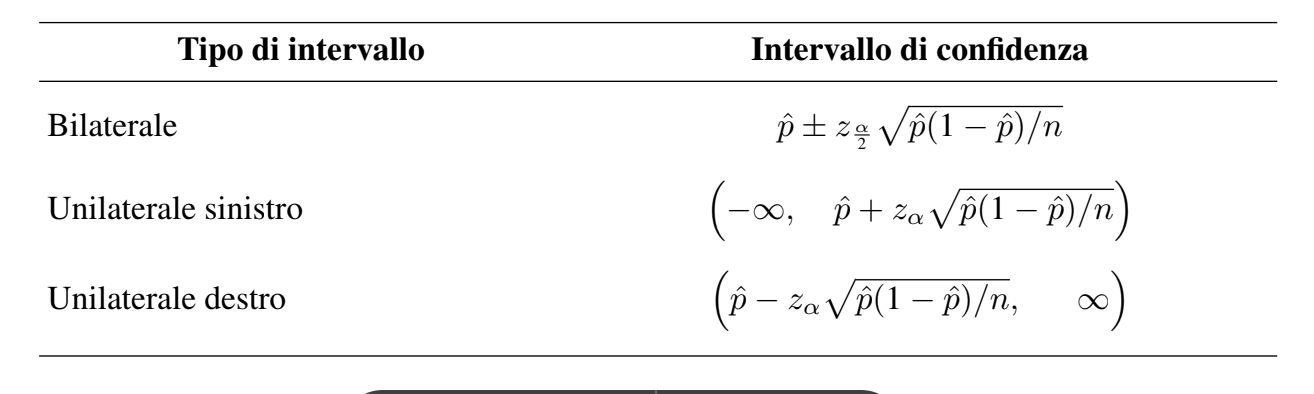
\includegraphics[width=\textwidth]{images/boh_3.png}
    \end{figure}
    \subsection{Metodo Montecarlo}
    supponendo di avere una funzione $f$ da $\mathbb{R}^r$ in $\mathbb{R}$ e vogliamo stimare la quantità $\theta$:
    \[ \theta := \int_{0}^{1} \int_{0}^{1} \cdots \int_{0}^{1} f(y_1, y_2, \ldots, y_n) \, dy_1 \, dy_2 \ldots \, dy_n \]
    Possiamo notare che $U_1, U_2, \ldots, U_r$ sono var. al. \textit{uniformi} su 0,1 quindi:
    \[ \ev{f(U_1, U_2, \ldots, U_r)} = \theta \]
    Se produciamo un numero casuale distribuito come la funzione e lo ripetiamo $n$ volte, possiamo stimare $\boldsymbol{\theta}$:
    \[ \hat{\theta} = \frac{1}{n} \sum_{i = 1}^{n} X_i \]
    \paragraph{Esempio} pensiamo alla stima di questo integrale:
    \[ \theta := \int_{0}^{1} \sqrt{1 - y^2} \, dy = \ev{\sqrt{1-U^2}} \]
    Se $\boldsymbol{U_1, U_2, \ldots, U_{100}}$ sono variabili aleatorie con tale distribuzione e \textit{indipendenti} ponendo:
    \[ X_i := \sqrt{1-U^2_i} \qquad i = 1,2, \ldots, 100 \]
    Otteniamo un campione di \textbf{100} variabili aleatorie di media $\theta$. \\ 
    Calcoliamo ora la \textit{media campionaria}:
    \[ \hat{\theta} = \frac{1}{n} \sum_{i=1}^{n} X_1 = 0.786 \]
    e successivamente la \textit{deviazione standard campionaria}:
    \[ S = 0.23 \]
    dato che $t_{0.025, 99} \approx 1.985$ otteniamo che un intervallo di confidenza al 95\% per $\theta$ è il seguente:
    \[ 0.786 \pm 1.985 \cdot 0.023 \]
    \centerline{Quindi il valore è compreso tra 0.740 e 0.832}
    \newpage
    \section{Intervalli di predizione}
    \subsection{Predizione di un elemento del mio campione}
    Supponiamo che $X_1, X_2, \ldots, X_n, X_{n+1}$ sia un campione normale con media $\mu$ e varianza $\sigma^2$ entrambe \textit{incognite}, dobbiamo prevedere l'elemento $X_{n+1}$ \\
    La sua distribuzione è:
    $$ \frac{X_{n+1}-\overline{X}}{\sigma\sqrt{1+\frac{1}{n}}} \sim t_{n-1} $$
    Dato che $\sigma$ è incognita dobbiamo sostituirla col suo stimatore (scegliendo la \textit{deviazione standard campionaria}) quindi poniamo:
    \[ S^2_n := \frac{1}{n -1} \sum_{i= 1}^{n} (X_i - \overline{X}_n)^2 \]
    \paragraph{quindi otteniamo}
    $$ X_{n+1} \in \Big(\overline{X}_n-t_{\frac{\alpha}{2}, n-1} S_n\sqrt{1+\frac{1}{n}},\overline{X}_n+t_{\frac{\alpha}{2}, n-1} S_n\sqrt{1+\frac{1}{n}}\Big) $$
    \paragraph{Esempio} prendiamo in campione i valori rilevati da un contapassi negli ultimi 7 giorni \\
    Dataset: \{ 6822 5333 7420 6252 7005 6752 \} \\
    Si trovi l'intervallo di predizione al 95\% di confidenza
    \paragraph{Risoluzione} cerchiamo le statistiche del campione ($X_{n+1}$):
    \[ \overline{X}_7 \approx 6716.57 \qquad \qquad S_7 \approx 733.97 \]
    Dalle tabelle ricaviamo che $t_{0.025,6} \approx 2.447$ (+ altri passaggi) concludiamo col dire che il 95\% di confidenza che $X_8$ cadrà nell'intervallo [4796, 8637]
    \newpage
    \section{Intervalli di confidenza per la varianza} 
    Se $X_1, X_2, \ldots, X_n$ un campione di una distribuzione \textit{normale} con parametri $\mu$ e $\sigma^2$ \textbf{incogniti}
    \formula \[ (n-1) \frac{S^2}{\sigma^2} \sim \mathcal{X}^2_{n-1}  \]
    \paragraph{Per caso Bilaterale}:
    \begin{equation}
        \left(\frac{(n-1) s^2}{\chi_{\frac{\alpha}{2}, n-1}^2}, \quad \frac{(n-1) s^2}{\chi_{1-\frac{\alpha}{2}, n-1}^2}\right)
    \end{equation}
    \paragraph{Per caso Unilaterale}:
    \begin{equation}
        \left( \sigma^2  < \frac{(n-1)S^2}{\mathcal{X}^2_{1-\alpha, n-1}}\right) \quad \left( \frac{(n-1)S^2}{\mathcal{X}^2_{\alpha, n-1}} < \sigma^2 \right)
    \end{equation}
    \begin{figure}[H]
        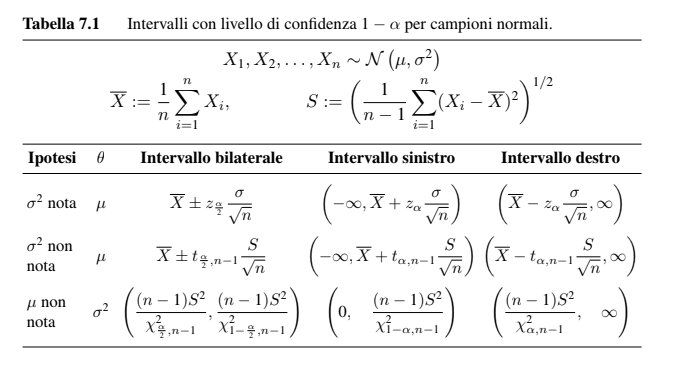
\includegraphics[width=\textwidth]{images/boh_2.png}
    \end{figure}
    \subsection{Stime per la differenza tra le medie di due popolazioni normali}
    Siano $X_1, X_2, \ldots, X_n$ e $Y_1, Y_2, \ldots, Y_m$ due campioni normali e differenti, denotiamo con $\mu_1$ e $\sigma^2_1$ e con $\mu_2$ e $\sigma^2_2$ le nostri variabili\\
    $\boldsymbol{\overline{X} - \overline{Y}}$ è lo stimatore di massima verosomiglianza $\mu_1 - \mu_2$ \\
    Per ottenere uno \textit{stimatore non puntuale}, dobbiamo \textbf{conoscere} la distribuzione di $\overline{X} - \overline{Y}$ poiche:
    \[ \overline{X} \sim \mathcal{N} \left( \mu_1, \frac{\sigma^2_1}{n} \right)  \qquad \text{e} \qquad \overline{Y} \sim \mathcal{N}\left( \mu_2, \frac{\sigma^2_2}{m} \right) \]
    Possiamo dedurre che:
    \[ \overline{X} - \overline{Y} \sim \mathcal{N}\left( \mu_1 - \mu_2, \frac{\sigma^2_1}{n} + \frac{\sigma^2_2}{m} \right) \]
    Ipotizzando di conoscere $\sigma^2_1$ e $\sigma^2_2$ abbiamo che:
    \[ \frac{\overline{X} - \overline{Y} - (\mu_1 - \mu_2)}{\sqrt{\sigma^2_1 / n + \sigma^2_2 / m}} \sim \mathcal{N}(0,1) \]
    e possiamo ulteriormente dedurre che
    \paragraph{Per caso Bilaterale}
    \begin{equation*}
        \begin{aligned}
            1-\alpha & =\left(-z_{\frac{\alpha}{2}}<\frac{\overline{X}-\overline{Y}-\left(\mu_1-\mu_2\right)}{\sqrt{\sigma_1^2 / n+\sigma_2^2 / m}}<z_{\frac{\alpha}{2}}\right) \\
            & =\left(\overline{X}-\overline{Y}-z_{\frac{\alpha}{2}} \sqrt{\frac{\sigma_1^2}{n}+\frac{\sigma_2^2}{m}}<\mu_1-\mu_2<\overline{X}-\overline{Y}+z_{\frac{\alpha}{2}} \sqrt{\frac{\sigma_1^2}{n}+\frac{\sigma_2^2}{m}}\right)
            \end{aligned}
    \end{equation*}
    \paragraph{Per caso Unilaterale}
    \begin{equation*}
        \begin{aligned}
            &\left( \overline{X} - \overline{Y} - z_{\alpha} \sqrt{\frac{\sigma^2_1}{n} + \frac{\sigma^2_2}{m}}< \mu_1 - \mu_2 \right) \\
            &\left( \mu_1 - \mu_2 < \overline{X} - \overline{Y} - z_{\alpha} \sqrt{\frac{\sigma^2_2}{n} + \frac{\sigma^2_2}{m}} \right) \\
           \end{aligned}
    \end{equation*}
    \begin{figure}[H]
        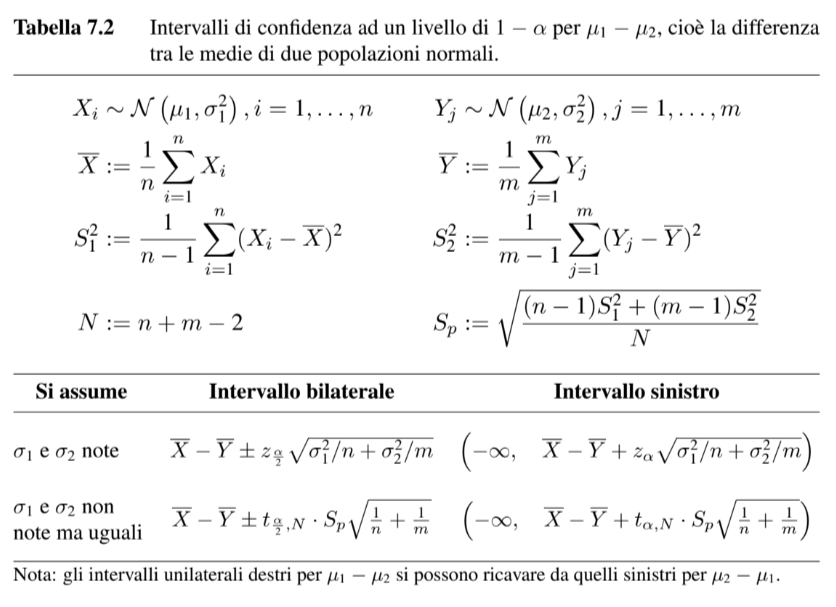
\includegraphics[width=\textwidth]{images/Screenshot_1.png}
    \end{figure}
    \section{Qualità ed efficienza degli stimatori}
    Sia $X := (X_1, X_2, \ldots, X_n)$ un campione di una distribuzione \textit{nota} tranne per il parametro $\theta$ che è incognito e $d(X)$ uno stimatore di $\theta$ \\
    Come possiamo valutare la sua efficacia? \\
    un criterio può essere quello dell'\textit{errore quadratico medio} ossia:
    \[ r(d, \theta) := \ev{(d(X) - \theta)^2} \]
    \centerline{sarà questo il nostro \textbf{indicatore} del valore di $d$ come stimatore di $\theta$}
    \subsection{Bias e Polarizzazione}
    \definizione Sia $d= d(X)$ uno stimatore del parametro $\theta$ allora:
    \[ b_\theta (d) := \ev{d(X)} - \theta \]
    \centerline{Questo viene detto \textit{bias} di d come stimatore di $\theta$} \\[2ex]
    Se il bias è nullo(quindi $\ev{d(X)} = \theta$), si dice che è uno stimatore \textit{corretto} o \textit{non distorto}
    \paragraph{Definizione} Sia $X_1, \ldots, X_n$ un campione con media \textit{incognita} $\theta$ quindi:
    \[ d_1 (X_1, X_2, \ldots, X_n) = X_1 \]
    \[ d_2 (X_1, X_2, \ldotp, X_n) = \frac{X_1 + X_2 + \cdots + X_n}{n} \]
    \centerline{sono entrambi \textit{stimatori non distorti di $\theta$}}
    la verifica è immediata:
    \[ \ev{X_1} = \ev{\frac{X_1 + X_2 + \cdots + X_n}{n}} = \theta \]
    \paragraph{Definizione} Se $d = d(X)$ è uno \textit{stimatore corretto}, il suo errore quadratico medio diventa:
    \begin{equation*}
        \begin{split}
            r(d, \theta) &= \ev{(d- \theta)^2} \\
            &= \ev{(d-\ev{d})^2} \\
            &= Var(d)
        \end{split}
    \end{equation*}
    \centerline{Quindi l'errore quadratico medio di uno stimatore corretto è \textbf{pari alla sua varianza}}
    \subsection{Combinazioni di stimatori corretti}
    Consideriamo due stimatori \textit{corretti} e \textit{indipendenti} di parametro $\theta$ (denotati con $d_1$ e $d_2$) con varianze rispettivamente $\sigma^2_1$ $\sigma^2_2$
    \[ \ev{d_i} = \theta \qquad Var(d_i) = \sigma^2_i \qquad i=1,2  \]
    uno stimatore corretto di $\theta$ è il seguente
    \[ d := \lambda d_1 + (1- \lambda) d_2 \]
    Successivamente vogliamo trovare anche il valore di $\lambda$ che produce lo stimatore $d$ con il \textit{minore errore quadratico medio}
    \begin{equation*}
        \begin{split}
            r(d, \theta) &= Var(d) \\
            &= \lambda^2 Var(d_1) + (1- \lambda)^2 Var(d_2) \qquad \text{per l'indipendenza di $d_1$ e $d_2$} \\
            &= \lambda^2 \sigma^2_1 + (1-\lambda)^2 \sigma^2_2
        \end{split}
    \end{equation*}
    ayo bro what's this shit, le me calculate the derivata with latti:
    \[ \frac{d}{d \lambda} r(d, \theta) = 2 \lambda \sigma^2_1 - 2(1- \lambda) \sigma^2_2 \]
    e belin lo studiamo sto segno o no? denotiamo con $\hat{\lambda}$ il valore di $\theta$ che produce il minimo
    \[ 2 \hat{\lambda} \sigma^2_1 - 2(1- \hat{\lambda}) \sigma^2_2 = 0 \]
    da cui otteniamo:
    \[ \boldsymbol{\hat{\lambda} = \frac{\sigma^2_2}{\sigma^2_1 + \sigma^2_2} = \frac{1 / \sigma^2_1}{1 / \sigma^2_1 + 1 / \sigma^2_2}} \]
    il peso ottimale da dare a uno stimatore deve essere \textbf{inversamente} proporzionale alla sua varianza \\
    La migliore combinazione lineare delle $d_i$ per l'errore quadratico medio è:
    \begin{equation*}
        \begin{split}
            r(d, \theta) &= Var(d) \\
            &= \left( \frac{1}{\sum_{i=1}^{n}} 1 / \sigma^2_i \right)^2 \sum_{i=1}^{n} \left( \frac{1}{\sigma^2_i} \sigma^2_i \right) \\
            &= \frac{1}{\sum_{i=1}^{n} 1 / \sigma^2_i}
        \end{split}
    \end{equation*}
    \[ r(d, \theta) = Var(d) \]
    \paragraph{Bias/Polarizzazione}
    Se $d(X)$ è \textbf{distorto}:
    \begin{equation*}
        \begin{split}
            r(d, \theta) &= \ev{(d - \theta)^2} \\
            &= Var(d) + 0 + \ev{b_\theta (d)^2} \\
            &= Var(d) + b_\theta(d)^2
        \end{split}
    \end{equation*}
    \begin{figure}[h]
        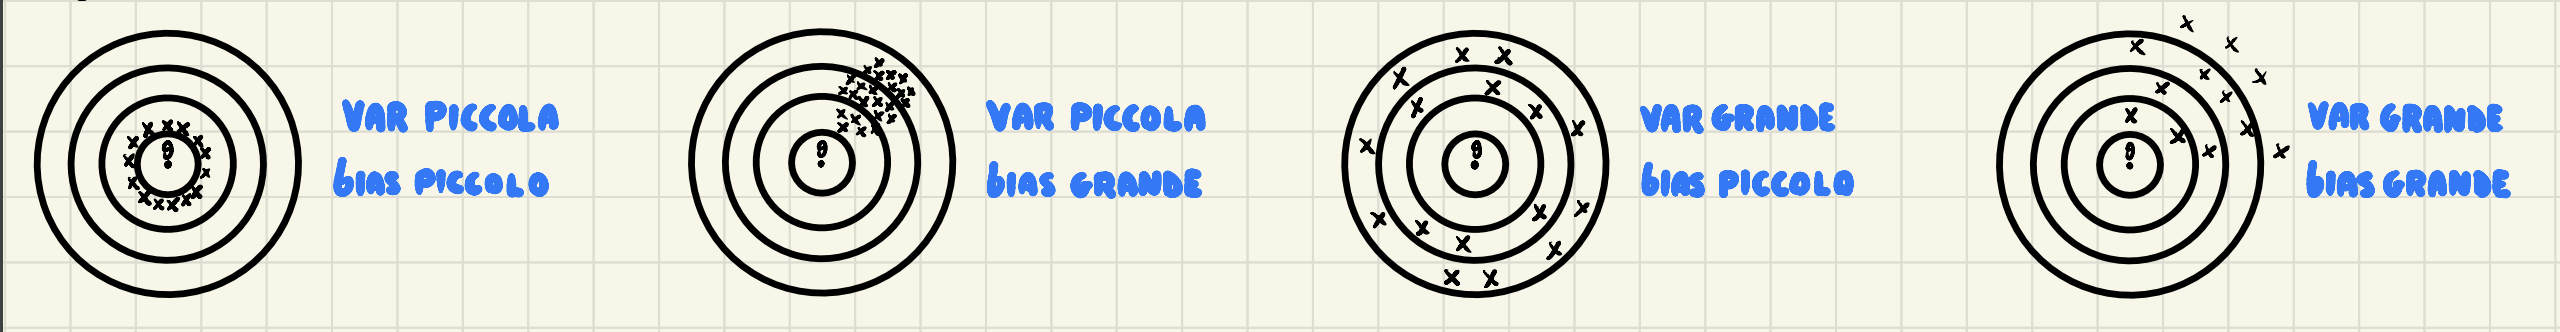
\includegraphics[width=\textwidth]{images/boh_4.png}    
    \end{figure}
    \subsection{Stimatore della media di una distribuzione uniforme}
    Siano $X_1, X_2, \ldots, X_n$ un campione estratto da una popolazione con distribuzione \textit{uniforme} su $(0, \theta)$ dove $\theta$ è un parametro incognito. \\
    Dato che $\boldsymbol{\ev{X_i} = \frac{\theta}{2}}$ è uno stimatore naturale per $\theta$ ed è dato da:
    \[ d_1 = d_1 (X) := 2 \overline{X} := \frac{2}{n} \displaystyle\sum_{i=1}^{n} X_i \]
    Siccome $\boldsymbol{\ev{d_1} = \theta}$, otteniamo che:
    \begin{equation*}
        \begin{split}
            \boldsymbol{r(d_1, \theta)} &= Var(d_1) \\
            &= \frac{4}{n} Var(X_i) \\
            &= \frac{4}{n} \cdot \frac{\theta^2}{12} \\
            &= \boldsymbol{\frac{\theta^2}{3n}}
        \end{split}
    \end{equation*}
    Un secondo stimatore che abbiamo è quello di \textbf{massima verosomiglianza} ($d_2$):
    \[ d_2 = d_2(X) = MLE := \max(X_i) \]
    Per trovare l'errore quadratico medio di $d_2$ dobbiamo prima conoscere la sua \textit{media} e la sua \textit{varianza}
    \[ \ev{d_2} = \int_{0}^{\theta} x \frac{nx^{n-1}}{\theta^n} \, dx = \frac{n}{n + 1} \theta \]
    \[ \ev{d^2_2} = \int_{0}^{\theta} x^2 \frac{nx^{n-1}}{\theta^n} \, dx = \frac{n}{n+2} \theta^2 \]
    \[ Var(d_2) = \ev{d^2_2} - \ev{d_2}^2 = \frac{n \theta^2}{(n+2) (n+1)^2} \]
    Quindi ora calcoliamo la $\boldsymbol{r(d_2, \theta)}$:
    \begin{equation}
        \begin{aligned}
        \boldsymbol{r\left(d_2, \theta\right)} & =\operatorname{Var}\left(d_2\right)+\left(E\left[d_2\right]-\theta\right)^2 \\
        & =\frac{n \theta^2}{(n+2)(n+1)^2}+\frac{\theta^2}{(n+1)^2} \\
        & =\frac{\theta^2}{(n+1)^2}\left[\frac{n}{n+2}+1\right] \\
        & =\frac{2 \theta^2}{(n+1)(n+2)}
        \end{aligned}
    \end{equation}
    Confrontando gli errori quadratici medi notiamo che $d_2$ è \textbf{migliore} di $d_1$ per $\theta$
    \[ \frac{2 \theta^2}{(n+1)(n+2)} \leq \frac{\theta^2}{3n} \qquad \text{$d_2$ migliore} \]
    \begin{figure}[H]
        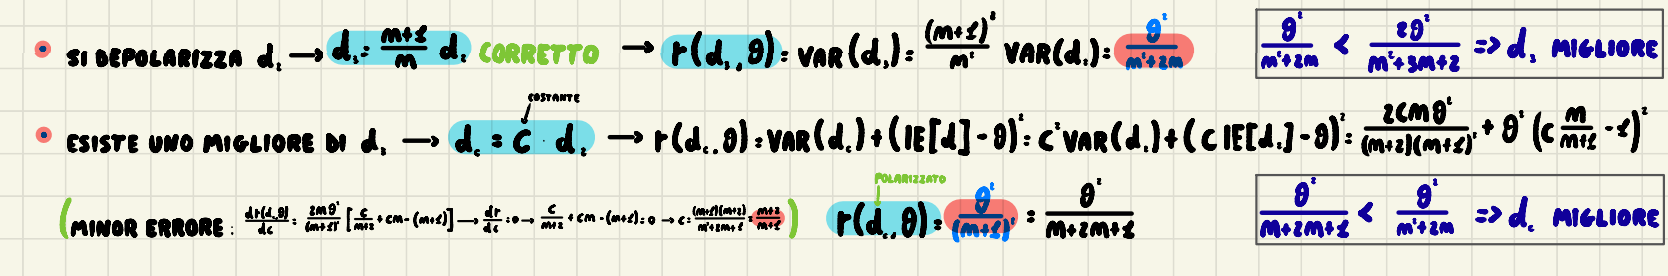
\includegraphics[width=\textwidth]{images/boh_5.png}
    \end{figure}
    \section{Stimatori Bayesiani}
    \definizione Quando il parametro incognito $\boldsymbol{\theta}$ possiamo considerarlo come una variabile aleatoria, questo approccio viene detto \textit{bayesiano} se abbiamo delle informazioni su quelli che possono essere assunti i valori da $\theta$ \\
    Esse assumono la forma di distribuzione di probabilità si dice che abbiamo \textbf{una distribuzione a priori per $\boldsymbol{\theta}$} \\[2ex]
    Se i valori che osserviamo sono $X_i = x_i \quad \text{e} \quad i=1,2, \ldots, n$ \\
    la \textit{densità di probabilità condizionale di $\theta$} è data da:
    \begin{equation*}
        \begin{split}
            \mathcolor{ForestGreen}{\boldsymbol{f(\theta \rvert x_1, x_2, \ldots, x_n)}} &= \frac{f(x_1, x_2, \ldots, x_n, \theta)}{\mathcolor{Turquoise}{\boldsymbol{f(x_1, x_2, \ldots, x_n)}}} \\
            &= \frac{\mathcolor{red}{\boldsymbol{f(x_1, x_2, \ldots, x_n \rvert \theta)}} \mathcolor{blue}{\boldsymbol{p(\theta)}}}{\int_{}^{} f(x_1, x_2, \ldots, x_n \rvert \theta') p(\theta') d\theta'}
        \end{split}
    \end{equation*}
    Dove:
    \begin{itemize}
        {\color{ForestGreen} \item $\boldsymbol{f(\theta \rvert x_1, x_2, \ldots, x_n)}$ Viene detta \textit{distribuzione a posteriori}}
        {\color{Turquoise} \item $\boldsymbol{f(x_1, x_2, \ldots, x_n)}$ è la \textit{MLE Marginale}}
        {\color{red} \item $\boldsymbol{f(x_1, x_2, \ldots, x_n \rvert \theta)}$ è la \textit{MLE}}
        {\color{blue} \item $\boldsymbol{p(\theta)}$ è la \textit{distribuzione a priori}}
    \end{itemize}
    Una buona stima per $\theta$ può essere la \textbf{media} perciò:
    \[ \ev{\theta \rvert X_1 = x_1, \ldots, X_n = x_n} = \int_{-\infty}^{\infty} \theta f(\theta \rvert x_1, x_2, \ldots, x_n) \, d\theta \quad \text{\textit{nel caso continuo}} \]
    \subsection{Stimatore di $\theta$ per Bernoulli}
    Se abbiamo $X_1, X_2, \ldots, X_n$ Bernoulliane, con massa di probabilità:
    \[ f(x \rvert \theta) = \theta^x (1-\theta)^{1-x} \qquad x = 0,1 \]
    \centerline{Dove $\theta$ è un parametro sconosciuto}
    Supponiamo quindi che la \textit{distribuzioni a priori} di $\theta$ sia uniforme su (0,1), denotiamo con $p$ la densità a propri di $\theta$
    \[ p(\theta)=1 \qquad 0 < \theta < 1 \]
    La densità condizionale di $\theta$ date $x_1, x_2, \ldots, x_n$ è 
    \begin{equation}
        \begin{aligned}
        f\left(\theta \mid x_1, x_2, \ldots, x_n\right) & =\frac{f\left(x_1, x_2, \ldots, x_n, \theta\right)}{f\left(x_1, x_2, \ldots, x_n\right)} \\
        & =\frac{f\left(x_1, x_2, \ldots, x_n \mid \theta\right) p(\theta)}{\int_0^1 f\left(x_1, x_2, \ldots, x_n \mid \vartheta\right) p(\vartheta) d \vartheta} \\
        & =\frac{\theta^{\sum_i x_i}(1-\theta)^{n-\sum_i x_i}}{\int_0^1 \vartheta^{\sum_i x_i}(1-\vartheta)^{n-\sum_i x_i} d \vartheta}
        \end{aligned}
    \end{equation}
    Non è difficile provare (e invece lo è) integrando per parti un certo numero di volte che per ogni valore di $m$ e $r$:
    \[ \int_{0}^{1} \theta^m (1-\theta)^r \, d\theta = \frac{m! r!}{(m+r+1)!} \]
    poniamo ora $\boldsymbol{x := \sum_{i=1}^{n} x_i}$
    \[ f(\theta \rvert x_1, x_2, \ldots, x_n) = \frac{(n+1)!}{x! (n-x)!} \theta^x (1-\theta)^{n-x} \qquad 0 < \theta < 1 \]
    Ora siamo in grado di calcolare \textit{la stima bayesiana}
    \begin{equation}
        \begin{aligned}
        E\left[\theta \mid x_1, x_2, \ldots, x_n\right] & =\frac{(n+1) !}{x !(n-x) !} \int_0^1 \theta^{1+x}(1-\theta)^{n-x} d \theta \\
        &=\frac{(n+1) !}{x !(n-x) !} \frac{(1+x) !(n-x) !}{(n+2) !} \\
        &= \frac{x+1}{n+2} \\
        &= \boldsymbol{\frac{1 + \sum_{i=1}^{n} x_i}{n + 2}}
        \end{aligned}
    \end{equation}
    \paragraph{Esempio} Se raccogliamo un campione di \textit{\textbf{10} bernoulliane} e trovassimo \textbf{6 successi}, lo stimatore bayesiano di $\theta$ fornirebbe un valore di \textbf{7 / 12} \\
    Lo stimatore di massima verosomiglianza vale invece \textbf{6 / 10}
    \subsection{Stimatore di $\theta$ per una Normale}
    Supponiamo che $X_1, X_2, \ldots, X_n$ sia una distribuzione normale con media $\theta$ \textit{incognita} e varianza $\sigma^2_0$ \textbf{nota} \\[2ex]
    Calcoliamo la \textit{densità condizionale} di $\theta$:
    \[ f(\theta \rvert x_1, x_2, \ldots, x_n) = \frac{f(x_1, x_2, \ldots, x_n \rvert \theta) p(\theta)}{f(x_1, x_2, \ldots, x_n)} \]
    Ora calcoliamo la \textit{media}:
    \[ \ev{\theta \rvert X_1, X_2, \ldots, X_n } = \boldsymbol{\frac{n / \sigma^2_0}{n / \sigma^2_0 + 1 / \sigma^2} \overline{X} + \frac{1 / \sigma^2}{n / \sigma^2_0 + 1 / \sigma^2} \mu} \]
    e successivamente la \textit{varianza}:
    \[ Var(\theta \rvert X_1, X_2, \ldots, X_n) = \boldsymbol{\frac{1}{n / \sigma^2_0 + 1 / \sigma^2}} \]
    \subsection{Stimatore di $\theta$ per Uniformi}
    Avendo una funzione di likelihood $f(x_1, x_2, \ldots, x_n \rvert \theta)$ e sapendo che la distribuzione è \textit{uniforme} \\
    $\theta \in [a,b]$ \\
    $d_b = d_{MLE}$
    \newpage
    \section{Verifica delle ipotesi}
    Un ipotesi statistica è un'affermazione su uno o più parametri della distribuzione, si chiama ipotesi perchè non sappiamo a priori se sia vera oppure no.
    \subsection{Livelli di significatività}
    Consideriamo una popolazione con distribuzione $F_\theta$ che dipende da $\theta$ incognito e vogliamo verificare una qualche ipotesi su questo parametro.
    \begin{enumerate}
        \item $H_0 : \theta = 1 \longrightarrow$ \textit{Ipotesi nulla \textbf{semplice}}
        \item $H_0 : \theta \leq n \longrightarrow$ \textit{Ipotesi nulla \textbf{composta}}
    \end{enumerate}
    Quando la prima ipotesi è vera, \textbf{caratterizza} l'intera distribuzione \\
    mentre questo non è vero per la seconda ipotesi. 
    \\[2ex]
    Esiste una regione critica \textbf{C} per cui se il campione aleatorio vi appartiene l'ipotesi \textit{non viene accettata}. \\
    Esiste un livello di tolleranza specificato all'interno della regione critica per cui un'ipotesi può essere \textit{ancora accettata}.
    Questa tolleranza è definita dal \textbf{livello di significatività}, ovvero viene definito $\alpha$ tale che se l'ipotesi è vera la probabilità di rifiutarla non superi $\alpha$:
    \[ \text{accetta } H_0 \text{ se} (X_1, X_2, \ldots, X_n) \not \in C \]
    \centerline{e}
    \[ \text{rifiuta } H_0 \text{ se} (X_1, X_2, \ldots, X_n) \in C \]
    Esistono \textbf{due tipi di errori}:
    \begin{enumerate}
        \item \textbf{Prima Specie}: Si rifiuta $H_0$ anche se è vera
        \item \textbf{Seconda Specie}: si accetta $H_0$ anche se è falsa
    \end{enumerate}
    \subsection{Verifica di ipotesi sulla media di una popolazione normale}
    Supponiamo che $X_1, X_2, \ldots, X_n$ sia un campione aleatorio di una popolazione normale di parametri $\mu$ $\sigma^2$ con \textit{varianza} nota e \textit{media} incognita, vogliamo verificare le seguenti ipotesi:
    \[ H_0 : \mu = \mu_0 \quad \text{ contro } \quad H_1 : \mu \not = \mu_0 \]
    Lo \textbf{stimatore puntuale} per $\mu$ è:
    \[ \overline{X} := \frac{1}{n} \sum_{i=1}^{n} X_i \]
    La \textbf{regione critica del test} invece è:
    \[ C := \{ (X_1, X_2, \ldots, X_n) : \rvert \overline{X} - \mu_0 \rvert > c \} \]
    \centerline{Dove c rappresenta la \textit{tolleranza}} \\[2ex]
    Quando $\mu = \mu_0$ sappiamo che $\overline{X}$ ha distribuzione \textbf{normale} con media $\mu_0$ e varianza $\sigma^2 / n$ allora:
    \[ \frac{\overline{X} - \mu_0}{\sigma / \sqrt{n}} \sim Z \]
    \centerline{Dove la relazione $\sim$ è \textbf{condizionata} all'ipotesi $H_0 : \mu = \mu_0$} \\[2ex]
    \textbf{c} deve soddisfare la seguente relazione:
    \[ \alpha = P(\text{errore di I specie}) = \boldsymbol{P_{\mu_0}(\rvert \overline{X} - \mu_0) > c} \]
    Possiamo scrivere l'equazione di sopra in questo modo:
    \[ \alpha = 2P \left( Z > \frac{c \sqrt{n}}{\sigma} \right) \]
    Per $P(Z > c \sqrt{n} / \sigma)$ per la definzione $z_{\frac{\alpha}{2}}$ vale:
    \[ P\left( Z > z_{\frac{\alpha}{2}} \right)= \frac{\alpha}{2} \longrightarrow c = z_{\frac{\alpha}{2}} \frac{\sigma}{\sqrt{n}}\]
    Il test con livello di significatività ha \textbf{due esiti}:
    \[ \text{si rifiuta } H_0 \text{ se} \bigg\rvert \frac{\overline{X} - \mu_0}{\sigma / \sqrt{n}} \bigg\rvert > z_{\frac{\alpha}{2}} \]
    \[ \text{si accetta } H_0 \text{ se} \bigg\rvert \frac{\overline{X} - \mu_0}{\sigma / \sqrt{n}} \bigg\rvert \leq z_{\frac{\alpha}{2}} \]
    p dei dati $= \sqrt{n} \frac{\overline{X} - \mu_0}{\sigma}$ \\[2ex]
    $H_0$ si \textbf{accetta} se $2P(Z > z_{\frac{\alpha}{2}}) \text{ è elevata}$ \\
    $H_0$ si \textbf{rifiuta} se $2P(Z > z_{\frac{\alpha}{2}}) \text{ è bassa}$ \\
    Perche se la probabilità che $Z$ sia $> z_{\frac{\alpha}{2}}$ è \textit{alta} allora il mio valore sarà vicino al mezzo e va bene. Se è basso allora è \textit{lontano} dal mezzo e non va bene.
    \paragraph{Esempio} supponiamo una media campionaria dei \textit{5} segnali ricevuti fosse \textit{8.5}:
    \[ \frac{\sqrt{n}}{\sigma} \rvert \overline{X} - \mu_0 \rvert = \frac{\sqrt{5}}{2} \cdot 0.5 \approx 0.559 \]
    Dato che:
    \[ P(|Z| > 0.559) = 2P(Z > 0.559) \approx 2 X 0.288 = 0.576 \]
    Otteniamo che il \textit{p-dei-dati} è 0.576 e quindi l'ipotesi nulla che il segnale inviato fosse \textbf{8}, che viene accettata per ogni $\alpha < 0.576$ \\
    Se avessimo ottenuto che $\overline{X} = 11.5$ il valore del \textit{p-dei-dati} sarebbe:
    \[ P \left( |Z| > \frac{\sqrt{5}}{2} \cdot 3.5 \right) \approx 2P(Z > 3.913) \approx 0.00005 \]
    Con un valore così piccolo, l'ipotesi che il messaggio fosse stato 8, \textbf{va rifiutata}. \\[3ex]
    Riprendendo il discorso degli errori di specie andiamo a vedere ora \textit{gli errori di \textbf{seconda specie}}. \\
    Rinfreschiamo la memoria, l'errore di seconda specie è quando \textit{si accetta $H_0$ anche se è falsa}, quindi:
    \[ \boldsymbol{\beta(\mu)} := P_\mu (\text{accettare } H_0) = \boldsymbol{P_\mu \left( -z_{\frac{\alpha}{2}} \leq \frac{\overline{X} - \mu_0}{\sigma / \sqrt{n}} \leq z_{\frac{\alpha}{2}}\right)}\]
    La funzione $\beta(\mu)$ è detta \textbf{curva OC} (\textit{curva operativa caratteristica}) e rappresenta la probabilità di accettare $H_0$ quando la media reale è $\mu$.
    \begin{figure}[H]
        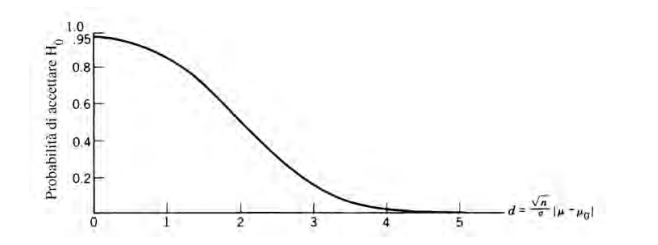
\includegraphics[width=\textwidth]{images/boh_6.png}
        \caption{Curva OC di un test \textit{bilaterale} per la media di una popolazione normale, con $\alpha = 0.05$}
    \end{figure}
    Per calcolare la probabilità ricordiamoci il fatto che $\overline{X} \sim \mathcal{N}(\mu, \sigma^2 / n)$:
    \[ Z := \frac{\overline{X} - \mu}{\sigma / \sqrt{n}} \sim \mathcal{N}(0,1) \]
    Quindi:
    \begin{equation*}
        \begin{split}
            \beta(\mu) &= P_\mu \left( -z_{\frac{\alpha}{2}} \leq \frac{\overline{X} - \mu_0}{\sigma / \sqrt{n}} \leq z_{\frac{\alpha}{2}} \right) \\
            &= \boldsymbol{\Phi \left( \frac{\mu_0 - \mu}{\sigma / \sqrt{n}} + z_{\frac{\alpha}{2}}\right) - \Phi \left( \frac{\mu_0 - \mu}{\sigma / \sqrt{n}} - z_{\frac{\alpha}{2}} \right) = 1 - \alpha}
        \end{split}
    \end{equation*}
    \centerline{Dove $\Phi$ indica la \textit{funzione di ripartizione} della distribuzione normale standard}
    \paragraph{Esempio} quanto vale la probabilità di accettare $\mu = 8$ quando in realtà $\mu = 10$:
    \[ \frac{\sqrt{n}}{\sigma} (\mu_0 - \mu) = \frac{\sqrt{5}}{2} (-2) = - \sqrt{5} \]
    Dato che $\boldsymbol{z_{0.025} \approx 1.96}$ ricaviamo la probabilità cercata:
    \begin{equation*}
        \begin{split}
            \beta(10) &\approx \Phi(- \sqrt{5} + 1.96) - \Phi(- \sqrt{5} - 1.96) \\
            &= 1 - \Phi(0.276) - 1 + \Phi(4.196) \\
            &\approx -0.609 + 1 = \boldsymbol{0.391}
        \end{split}
    \end{equation*}
    Riprendendo il discorso della curva OC, ci permette di dimensionare il campione in modo che \textit{l'errore di seconda specie} soddisfi le condizioni specifiche. \\[2ex]
    Come facciamo a trovare $n$ tale che la probabilità di \textit{accettare} $H_0 : \mu = \mu_0$ quando il vero valore è $\mu_1$ sia un valore fissato $\beta$ per $n$ tale che $\boldsymbol{\beta(\mu_1) \approx \beta}$
    \[ n \approx \left[ \frac{(z_{\frac{\alpha}{2}} + z_\beta) \sigma}{\mu_1 - \mu_0} \right]^2 \]
    \centerline{Notiamo che anche nel caso in cui $\boldsymbol{\mu_1 < \mu_0}$ troviamo sempre la stessa formula}
    \paragraph{Esempio} Quante volte è necessario inviare il segnale con verifica dell'ipotesi $H_0 : \mu = 8$ con livello di significatività 0.05 con almeno il 75\% di probabilità di rifiutare l'ipotesi nulla quando $\boldsymbol{\mu = 9.2}$ \\
    Dato che $z_{0.025 \approx 1.96}$ e $z_{0.25} \approx 0.67$ 
    \[ n \approx \left( \frac{1.96 + 0.67}{1.2} \right)^2 \cdot 4 \approx 19.21 \]
    Come vediamo per il risultato è necessario un \textit{campione di 20 segnali}, quindi con $n=20$
    \begin{equation*}
        \begin{split}
            \beta(9.2) &\approx \Phi \left( - \frac{1.2 \sqrt{20}}{2} + 1.96 \right) - \Phi \left( - \frac{1.2 \sqrt{20}}{2} - 1.96 \right) \\
            &\approx \Phi(-0.723) - \Phi(-4.643) \\
            &\approx 1 - \Phi(0.723) \approx \boldsymbol{0.235}
        \end{split}
    \end{equation*}
    Quindi ricapitolando, se il segnale viene trasmesso 20 volte c'è il 76.5\% di probabilità che l'ipotesi nulla $\mu = 8$ sia \textbf{rifiutata} se la media reale è \textbf{9.2}

    \subsection{Test unilaterali}
    Introduzione bla bla bla \\
    Verifichiamo due ipotesi:
    \[ H_0 : \mu = \mu_0 \quad \text{ contro } \quad H_1 : \mu > \mu_0 \]
    Dovremmo rifiutare l'ipotesi nulla quando lo stimatore di $\mu$ è molto più grande di $\mu_0$, la regione critica è quindi:
    \[ C := \{ (X_1, X_2, \ldots, X_n) : \overline{X} - \mu_0 > c \} \]
    la probabilità di rifiuto dovrebbe essere $\alpha$ quando $H_0$ è vera, occorre però che \textit{c} soddisfi la relazione:
    \[ P_{\mu_0} (\overline{X} - \mu_0 > c) = \alpha \]
    Il test \textit{con livello di significatività} $\alpha$ dovrà rifiutare $\boldsymbol{H_0 \text{ se } \overline{X} - \mu_0 > z_\alpha \cdot \sigma / \sqrt{n}}$
    \[ \text{si rifiuta } H_0 \text{ se} \frac{\overline{X} - \mu_0}{\sigma / \sqrt{n}} > z_\alpha \]
    \[ \text{si accetta } H_0 \text{ se} \frac{\overline{X} - \mu_0}{\sigma / \sqrt{n}} \leq z_\alpha \]
    Quella trovata è detta \textit{regione criticia \textbf{unilaterale}} o a una coda, quindi il problema di verificare le ipotesi alternative
    \[ H_0 : \mu = \mu_0 \quad \text{ contro } \quad H_1 : \mu > \mu_0 \]
    \centerline{Si dice problema di \textbf{test unilaterale}} \\[2ex]
    poniamo $Z := \sqrt{n}(\overline{X} - \mu) / \sigma$ questa statistica è una \textit{normale standard} quindi:
    \begin{equation*}
        \begin{split}
            \beta(\mu) &:= P_\mu(\text{accettare } H_0) \\
            &= P_\mu \left( Z \leq \frac{\mu_0 - \mu}{\sigma / \sqrt{n}} + z_\alpha \right) \\
            &= \boldsymbol{\Phi \left( \frac{\mu_0 - \mu}{\sigma / \sqrt{n}} + z_\alpha \right) = 1 - \alpha}
        \end{split}
    \end{equation*}
    Dato che $\Phi$ in quanto \textit{funzione di ripartizione è \textbf{crescente}} però $\beta(\mu)$ è una funzione \textbf{decrescente} \\
    L'ipotesi \textit{unilaterale}
    \[ H_0 : \mu \leq \mu_0 \]
    contro l'alternativa
    \[ H_1 : \mu > \mu_0 \]
    Per accertarci che il \textit{livello di significatività} sia rimasto $\alpha$ \\
    Al variare di $\mu$ la probabilità di rifiuto è data da $\boldsymbol{1 - \beta(\mu)}$ \\
    Dobbiamo verificare che per ogni $\mu$ compatibile con $H_0$ per ogni $\boldsymbol{\mu \leq \mu_0}$ 
    \[ 1 - \beta(\mu) \leq \alpha, \qquad \text{per ogni } \mu \leq \mu_0 \]
    Quindi:
    \[ \beta(\mu) \geq 1 - \alpha, \qquad \text{per ogni } \mu \leq \mu_0 \]
    \paragraph{Osservazione} è possibile verificare l'ipotesi
    \[ H_0 : \mu = \mu_0 \]
    \centerline{contro l'ipotesi \textit{alternativa}}
    \[ H_1 : \mu < \mu_0 \]
    ad un livello di significatività $\boldsymbol{\alpha}$, decidendo che:
    \[ \text{si rifiuta } H_0 \text{ se } \frac{\overline{X} - \mu_0}{\sigma / \sqrt{n}} \leq -z_\alpha \]
    \[ \text{si accetta } H_0 \text{ se } \frac{\overline{X} - \mu_0}{\sigma / \sqrt{n}} \geq -z_\alpha \]
    \subsection{Il test t}
    Fino ad ora abbiamo supposto che l'unico parametro incognito fosse la \textit{media}, in questo caso la nostra varianza $\boldsymbol{\sigma^2}$ \textbf{non è nota} \\
    In questa situazione consideriamo che si possa verificare l'ipotesi nulla che $\mu$ sia uguale ad un valore assegnato $\mu_0$ contro l'ipotesi alternativa $\mu \not= \mu_0$
    \[ H_0 : \mu = \mu_0 \]
    \[ H_1 : \mu \not= \mu_0 \]
    (Cambiare poi con desc più corta)
    Come in precedenza, sembra ragionevole rifiutare l’ipotesi nulla quando $\overline{X}$ cade
    lontano da $\mu_0$ tuttavia la distanza a cui deve essere da $\mu_0$ per giustificare questo
    rifiuto, dipende dalla deviazione standard $\sigma$ che in quella sede era nota; in particolare
    $|\overline{X} - \mu0|$ doveva essere maggiore di $z_{\frac{\alpha}{2}} \cdot \sigma / \sqrt{n}$ o equivalentamente
    \[ \left[ \frac{\overline{X} - \mu_0}{\sigma / \sqrt{n}} \right] > z_{\frac{\alpha}{2}} \]
    Qui $\boldsymbol{\sigma}$ non è più conosciuta, sostituiamola quindi con la \textit{deviazione standard campionaria} $S$
    \[ S := \sqrt{\frac{1}{n-1} \sum_{i=1}^{n} (X_i - \overline{X})^2} \]
    rifiutando l'ipotesi nulla quando 
    \[ \big\rvert \frac{\overline{X} - \mu_0}{S / \sqrt{n}} \big\rvert \] 
    Quindi alla fine noi dobbiamo ottenere una distribuzione t
    \[  t_{n-1} \sim \frac{\overline{X} - \mu}{S/ \sqrt{n}} \]
    Se si denota con T la statistica di questo test, ovvero 
    \[ T := \frac{\overline{X} - \mu_0}{S / \sqrt{n}} \]
    allora quando $H_0$ è vera (visto che $\mu = \mu_0$) ha distribuzione \textbf{$t$ con $n-1$ gradi di libertà.}
    \[ P_{\mu_0} \left( - c \leq \frac{\overline{X} - \mu_0}{S / \sqrt{n}} \leq c \right) = \boldsymbol{1- \alpha} \]
    Se vogliamo ricavare c:
    \begin{equation*}
        \begin{split}
            \alpha &= 1 - P(-c \leq T < c) \\
            &= P(T \leq -c) + P(T \geq c) \\
            &= 2P(T \geq c)
        \end{split}
    \end{equation*}
    Per cui $P(T > c) = \frac{\alpha}{2}$, e quindi deve valere $c = t_{\frac{\alpha}{2}, n-1}$, quindi in fin dei conti:
    \[ \text{si rifiuta } H_0 \text{ se } \big| \frac{\overline{X} - \mu_0}{S / \sqrt{n}} \big| > t_{\frac{\alpha}{2}, n-1} \]
    \[ \text{si accetta } H_0 \text{ se } \big| \frac{\overline{X} - \mu_0}{S / \sqrt{n}} \big| \leq t_{\frac{\alpha}{2}, n-1} \]
    \centerline{Vedere tabella sotto per tutt'e cose}
    \begin{figure}[H]
        \caption{$X_1, X_2, \ldots, X_n$ è un campionare estratto da una popolazione $\mathcal{N}(\mu, \sigma^2)$}
        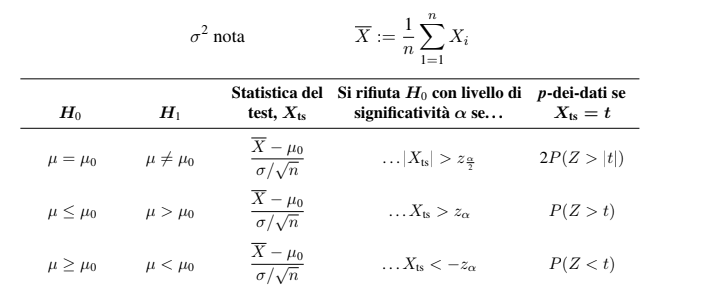
\includegraphics[width=\textwidth]{images/boh_7.png}
    \end{figure}
    \paragraph{Esempio} Vogliamo verificare l'ipotesi che il consumo \textit{medio} di acqua sia \textit{350} galloni al giorno. \\
    Si misurano i consumi medi di un campione di \textit{20 campioni} che seguono:
    \begin{figure}[H]
        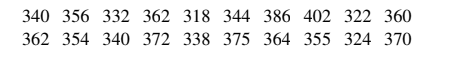
\includegraphics[width=\textwidth]{images/boh_8.png}
    \end{figure}
    Dobbiamo verificare le due ipotesi seguenti:
    \[ H_0 : \mu = 350 \quad \text{contro} \quad H_1 : \mu \not = 350 \]
    Calcoliamo ora la \textbf{media} e la \textbf{deviazione standard campionaria}
    \[ \overline{X} = 353.8 \qquad S \approx 21.85 \]
    troviamo ora il valore della statistica del test:
    \[ T \approx \frac{\sqrt{20} \cdot 3.8}{21.85} \approx 0.778 \]
    il valore che abbiamo trovato è minore di $t_{0.05, 19} \approx 1.729$ l'ipotesi nulla è \textit{accettata} ad un livello del \textit{5\%}
    TODO FINIRE PAGINA PDF 324 / 342 TOTALE
    \begin{figure}[H]
        \caption{$X_1, X_2, \ldots, X_n$ è un campionare estratto da una popolazione $\mathcal{N}(\mu, \sigma^2)$ e $\sigma^2$ non è nota}
        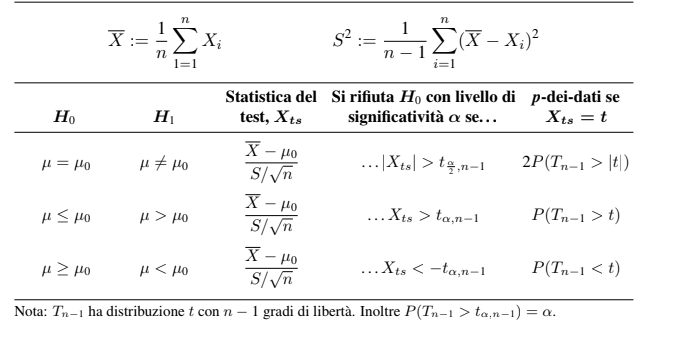
\includegraphics[width=\textwidth]{images/boh_9.png}
    \end{figure}
    \subsection{Verifica se due popolazioni hanno la stessa media}
    Una situazione che accade spesso è decidere se \textit{vari approcci} portano allo stesso risultato, oppure no. \\
    Questa problematica si ricordune spesso alla verifica dell'ipotesi che due popolazioni normali \textit{abbiano la stessa media.}
    \subsubsection{Il caso in cui le varianze sono note}
    Supponiamo che $X_1, X_2, \ldots, X_n$ e $Y_1, Y_2, \ldots, Y_n$ siano due campioni di due popolazioni \textit{normali} di medie $\mu_x$ $\mu_y$ e varianze \textit{note} $\sigma^2_x$ e $\sigma^2_y$ \\
    Come sempre verifichiamo le due ipotesi
    \[ H_0 : \mu_x = \mu_y \quad \text{ contro } \quad H_1 : \mu_x \not = \mu_y \]
    Dato che $\overline{X}$ e $\overline{Y}$ sono rispettivamente \textit{stimatori} di $\mu_x$ e $\mu_y$ \\
    Possiamo dire che $\overline{X} - \overline{Y}$ può essere \textbf{usato come stimatore} di $\mu_x - \mu_y$
    \[ \text{si rifiuta } H_0 \text{ se } \big|\overline{X} - \overline{Y} \big| > c \]
    \[ \text{si accetta } H_0 \text{ se } \big|\overline{X} - \overline{Y} \big| \leq c \]
    Come facciamo sempre noi possiamo trovare il valore di $c$ che rende questo test di livello di significatività $\alpha$ in questo modo:
    \[ \frac{\overline{X} - \overline{Y} - (\mu_x - \mu_y)}{\sqrt{\sigma^2_x / n + \sigma^2_y / m}} \sim \mathcal{N}(0,1) \]
    Per verificare l'ipotesi nulla $H_0 : \mu_x = \mu_y$ contro $H_1 : \mu_x \not = \mu_y$ facciamo cosi:
    \[ \text{si rifiuta } H_0 \text{ se } \frac{|\overline{X} - \overline{Y}|}{\sqrt{\sigma^2_x / n + \sigma^2_y / m}} > z_{\frac{\alpha}{2}} \]
    \[ \text{si accetta } H_0 \text{ se } \frac{|\overline{X} - \overline{Y}|}{\sqrt{\sigma^2_x / n + \sigma^2_y / m}} \leq z_{\frac{\alpha}{2}} \]
    \subsubsection{Il caso in cui le varianze non sono note ma supponiamo siano uguali}
    Prendiamo in considerazione i campioni di prima, tutti i nostri parametri sono \textit{incogniti} e studiamo le due ipotesi
    \[ H_0 : \mu_x = \mu_y \quad \text{ contro } \quad H_1 : \mu_x \not = \mu_y \]
    Prima di far tutto possiamo supporre che le due varianze \textit{incognite} siano uguali tra di loro quindi:
    \[ \sigma^2 := \sigma^2_x = \sigma^2_y \]
    Calcoliamo le due \textit{varianze campionarie}
    \[ S^2_x = \frac{1}{n-1} \sum_{i=1}^{n} (X_i - \overline{X})^2 \]
    \[ S^2_y = \frac{1}{m-1} \sum_{j=1}^{m} (X_j - \overline{Y})^2 \]
    Equazione idk:
    \[ \frac{\overline{X} - \overline{Y} - (\mu_x - \mu_y)}{S_p \sqrt{1 / n + 1 / m}} \sim t_{n+m-2}\]
    Dove $\boldsymbol{S^2_p}$ è lo \textit{stimatore pooled} di $\sigma^2$ e viene definito in questo modo:
    \[ S^2_p := \frac{(n-1) S^2_x + (m-1) S^2_y}{n + m -2} \]
    Quando $H_0$ è vera ($\mu_x - \mu_y = 0$):
    \[ T := \frac{\overline{X} - \overline{Y}}{S_p \sqrt{1 / n + 1 /m}} \]
    \centerline{ha distribuzione $t$ con $n + m - 2$ gradi di libertà} \\[2ex]
    Quindi possiamo verificare le ipotesi cosi:
    \[ \text{si rifiuta } H_0 \text{ se }  |T| > t_{\frac{\alpha}{2};n+m-2} \]
    \[ \text{si accetta } H_0 \text{ se }  |T| \leq t_{\frac{\alpha}{2};n+m-2} \]
    possiamo eseguire il test determinando \textit{il p-dei-dati}, denotando con $\upsilon$ il valore assunto da $T$
    \begin{equation*}
        \begin{split}
            \boldsymbol{p-dei-dati} &= P(|T_{n+m-2}| \geq |\upsilon|) \\
            &= 2P(T_{n+m-2} \geq |\upsilon|)
        \end{split}
    \end{equation*}
    \paragraph{Caso unilaterale}
    Per l'ipotesi \textit{unilaterale} abbiamo le due seguenti ipotesi:
    \[ \mu_0 : \mu_x \leq \mu_y \qquad \text{ contro } \qquad H_1 : \mu_x > \mu_y \]
    $H_0$ deve essere \textbf{rifiutata} per valore elevati di $T$, il test di significatività $\alpha$ è:
    \[ \text{si rifiuta } H_0 \text{ se }  T > t_{\alpha, n + m -2} \]
    \[ \text{si accetta } H_0 \text{ se }  T \leq t_{\alpha, n + m -2} \]
    il \textit{p-dei-dati} invece è il seguente (ricordando che $\upsilon$ è il valore assunto da $T$)
    \[ \boldsymbol{p-dei-dati} = P(T_{n+m-2} \geq \upsilon) \]
    \paragraph{Esempio} abbiamo $\overline{X} = 6.450$ e $\overline{Y} = 7.125$ \\
    Calcoliamo le due S, quindi $\boldsymbol{S^2_x \approx 0.581}$ e $\boldsymbol{S^2_y \approx 0.778}$ \\
    Calcoliamo ora lo stimatore $\boldsymbol{S^2_p}$:
    \[ S^2_p = \frac{9}{20} S^2_x + \frac{11}{20} S^2_y \approx 0.689 \]
    e la statistica del test:
    \[ \upsilon = \frac{-0.675}{\sqrt{0.689 ( 1/10 + 1/12)}} \approx -1.90 \]
    \subsubsection{verifica di due popolazioni con stessa media}
    \begin{figure}[H]
        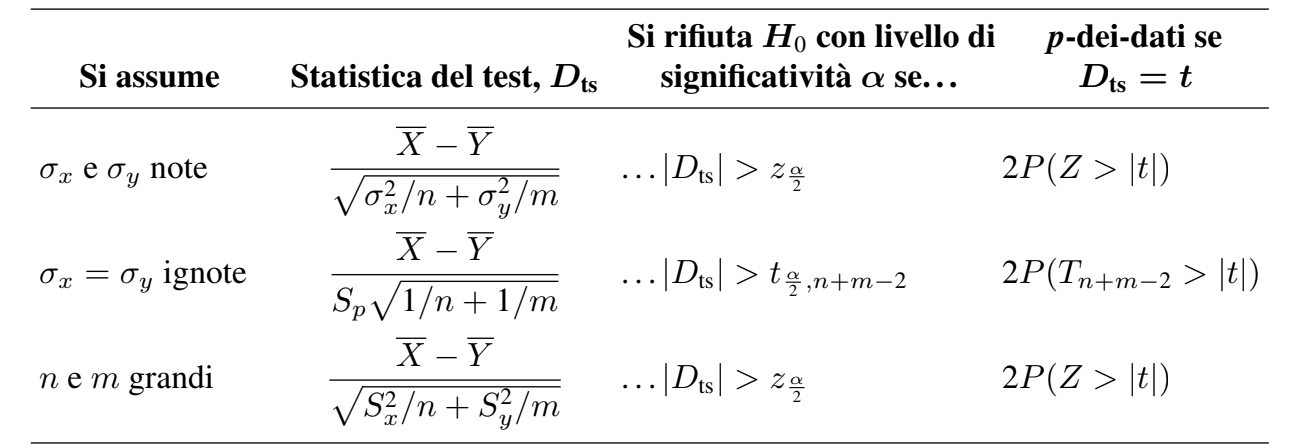
\includegraphics[width=\textwidth]{images/boh_10.png}
    \end{figure}
    \subsection{Il test t per campioni di coppie di dati}
    I dati che prendiamo in esempio sono descritti da $n$ coppie di valori $(X_i, Y_i)$ per $i = 1,2,\ldots, n$ \\
    $X_1, X_2, \ldots, X_n \qquad Y_1, Y_2, \ldots, Y_m \qquad$ \textbf{$n$ e $m$ devono essere uguali} \\ 
    Le nostre due variabili sono \textbf{dipendenti} quindi:
    \[ X \sim \mathcal{N}(\mu_x, \sigma_x) \]
    \[ Y \sim \mathcal{N}(\mu_y, \sigma_y) \]
    Se poniamo $\boldsymbol{W_i := X_i - Y_i}$ per $i=1,2,\ldots,n$ possiamo verificare queste due ipotesi
    \[ H_0 : \mu_W = 0 \quad \text{ contro } \quad H_1 : \mu_W \not = 0 \]
    La nostre $W$ provengono da un campione di popolazione $\mathcal{N}(\mu_W, \sigma^2_W)$, il test t quindi ci fornisce le seguenti regole:
    \[ \text{si accetta } H_0 \text{ se } - t_{\frac{\alpha}{2}, n-1} \leq \sqrt{n} \frac{\overline{W}}{S_W} \leq t_{\frac{\alpha}{2}, n-1} \]
    \[ \text{si rifiuta } H_0 \text{ negli altri casi} \]
    \subsection{Verifica di ipotesi sulla varianza di una popolazione normale}
    Sia $X_1, X_2, \ldots, X_n$ un campione di popolazione normale con media incognita $\mu$ e varianza incognita $\sigma^2$, verifichiamo le seguenti ipotesi:
    \[ H_0 : \sigma^2 = \sigma^2_0 \quad \text{ contro l'alternativa } \quad H_1 : \sigma^2 \not = \sigma^2_0 \]
    \centerline{con un valore di $\boldsymbol{\sigma^2_0}$ prefissato} \\[2ex]
    Otteniamo ora il test, abbiamo una distribuzione \textit{chi-quadro} con $n-1$ gradi di libertà, quindi quando $H_0$ è vera:\
    \[ \frac{S^2}{\sigma^2_0}(n-1) \sim \mathcal{X}^2_{n-1} \]
    e quindi otteniamo:
\    \[ P_{H_0} \left( \mathcal{X}^2_{1- \frac{\alpha}{2}, n-1} \leq \frac{S^2}{\sigma^2_0} (n-1) \leq \mathcal{X}^2_{\frac{\alpha}{2}, n -1} \right) = 1 - \alpha \]
    Queste sono infine le nostre regole da adottare
    \[ \text{si accetta } H_0 \text{ se } \mathcal{X}^2_{1-\frac{\alpha}{2}, n-1} \leq \frac{S^2}{\sigma^2_0} (n-1) \leq \mathcal{X}^2_{\frac{\alpha}{2}, n-1} \]
    \[ \text{si rifiuta } H_0 \text{ negli altri casi} \]
    Il \textit{p-dei-dati} del test è il seguente:
    \[ \boldsymbol{p-dei-dati} = 2 \min \{P(\mathcal{X}^2_{n-1} \leq c), \quad 1-P(\mathcal{X}^2_{n-1} \leq c)\} \]
    \subsection{Verifica di due popolazione normali che hanno la stessa varianza}
    Abbiamo $X_1, X_2, \ldots, X_n$ e $Y_1, Y_2,\ldots, Y_m$ sono due campioni \textit{normali} \textbf{indipendenti}, con $\mu_x, \sigma^2_x \quad$ e $\quad \mu_y, \sigma^2_y$ incogniti, vediamo le verifiche dell'ipotesi:
    \[ H_0 : \sigma^2_x = \sigma^2_y \quad \text{ contro } \quad H_1 : \sigma^2_x \not = \sigma^2_y \]
    Le due \textit{varianza campionarie} sono:
    \[ S^2_x = \frac{1}{n-1} \sum_{i=1}^{n} (X_i - \overline{X})^2 \]
    \[ S^2_y = \frac{1}{m-1} \sum_{j=1}^{m} (Y_j - \overline{Y})^2 \]
    Abbiamo una distribuzione F con parametri $n-1$ e $m-1$ quando $H_0$ è vera:
    \[ \frac{S^2_x}{S^2_y} \sim F_{n-1, m-1} \]
    e ne deduciamo che:
    \[ P_{H_0} \left( F_{1- \frac{\alpha}{2}, n-1, m-1} \leq \frac{S^2_x}{S^2_y} \leq F_{\frac{\alpha}{2}, n-1, m-1} \right) = 1 - \alpha \]
    Le nostre regole da adottare sono:
    \[ \text{si accetta } H_0 \text{ se } F_{1-\frac{\alpha}{2}, n-1, m-1} \leq \frac{S^2_x}{S^2_y} \leq F_{\frac{\alpha}{2}, n-1, m-1} \]
    \[ \text{si rifiuta } H_0 \text{ negli altri casi} \]
    Il test del \textit{p-dei-dati} è dato da:
    \[ \boldsymbol{p-dei-dati} = 2\min \{ P(F_{n-1,m-1} \leq \upsilon), \quad 1-P(F_{n-1,m-1} \leq \upsilon )\} \]
    \paragraph{Nota:} il test \textbf{impone} di rifiutare $H_0$ ogni volta che il \textit{livello di significatività} $\alpha$ è \textit{maggiore o uguale} al p-dei-dati
    \paragraph{Esempio} Vengono eseguiti 10 esperimenti nel primo caso e 12 nel secondo, con le seguenti varianze campionarie $S^2_1 = 0.14$ e $S^2_2 = 0.28$, possiamo rifiutare ad un livello di significatività del 5\% ? \\
    Calcoliamo la funzione di ripartizione delle \textit{distribuzioni F}, quindi:
    \[ P(F_{9,11} \leq 0.5) \approx 0.154 \]
    Quindi ora calcoliamo il \textit{p-dei-dati}
    \[ p-dei-dati \approx 2 \min(0.154, 0.846) = 0.308 \]
    \centerline{L'ipotesi nulla \textbf{deve essere accettata. }}
    \subsection{La verifica di ipotesi su una popolazione di Bernoulli}
    Il numero di difetti in un campione di $n$ pezzi ha una distribuzione \textit{binomiale} di parametri $(n, p)$, le verifiche dell'ipotesi sono le seguenti:
    \[ H_0 : p \leq p_0 \quad \text{ contro l'alternativa } \quad H_1 : p > p_0 \]
    \centerline{$p_0$ è un \textit{valore assegnato}}
    \[ \ev{X} = np \]
    \[ Var(X) = np (1-p) \]
    \[ \frac{X - np}{\sqrt{np_0 (1- p_0)}} \sim \mathcal{N}(0,1) \]
    --------------
    \[ \text{si accetta } H_0 \text{ se } \frac{X - np_0}{\sqrt{np_0 (1- p_0)}} \leq z_\alpha \]
    \[ \text{si rifiuta } H_0 \text{ se } \frac{X - np_0}{\sqrt{np_0 (1- p_0)}} > z_\alpha \]
    \section{AN.O.VA} 
    \definizione Analysis of variance, ci serve per confrontare più gruppi diversi per esempio per capire se hanno \textit{medie uguali}
    \[ Z_i := \frac{X_i - \mu_i}{\sigma^2} \sim \mathcal{N}(0,1) \]
    \centerline{le seguenti variabili aleatorie sono \textit{normali standard} e quindi:} \\[2ex]
    Abbiamo $m$ gruppi formati da $n$ oggetti. ogni gruppo rappresenta una variabile aleatoria $X_i \sim \mathcal{N}(\mu, \sigma^2)$
    \[ \sum_{i=1}^{N} Z^2_i = \sum_{i=1}^{N} \frac{(X_i - \mu_i)^2}{\sigma^2} \sim \mathcal{X}^2_N \]
    Essa è una \textit{chi-quadro} con $N$ gradi di libertà, non stimiamo direttamente le $\mu_i$ ma usiamo il fatto che queste sono combinazione lineari di $k$ \textit{parametri incogniti} \\
    In questa ipotesi possiamo dimostrare ciò:
    \[ \sum_{i=1}^{N} \frac{(X_i - \hat{\mu_i})^2}{\sigma^2} \sim \mathcal{X}^2_{N-k} \]
    \centerline{dove \textit{N} sono gli oggetti totali mentre \textit{k} sono i gruppi} \\[2ex]
    Prendiamo $\mu$ come \textit{unico parametro da stimare} cosi che $k=1$ se sostituiamo $\mu$ con $\overline{X}$ che è il suo stimatore, troviamo questa espressione:
    \[ \sum_{i=1}^{N} \frac{(X_i - \overline{X})^2}{\sigma^2} = \frac{N-1}{\sigma^2} \cdot \frac{1}{N-1} \sum_{i=1}^{N}(X_i - \overline{X})^2 = \boldsymbol{\frac{S^2}{\sigma^2}(N-1)} \]
    \subsection{Anova a 1 via}
    In questo caso noi abbiamo $m$ campioni \textit{indipendenti}, formati da $n$ variabili aleatorie con media che \textbf{dipende} dal campione e varianza \textit{fissata} \\
    Denotiamo $X_{ij} \quad i = 1,\ldots, m$ con quello che indica il campione mentre con $j=1, \ldots, n$ indichiamo la posizione all'interno del campione stesso \\[2ex] 
    I parametri $\mu_1, \mu_2, \ldots, \mu_m$ e $\sigma$ sono incogniti, il nostro scopo è quello di verificare l'ipotesi nulla:
    \[ H_0 : \mu_1 = \mu_2 = \cdots = \mu_m \quad \text{ contro } \quad H_1 : \mu_1 \not= \mu_2 \not= \cdots \not= \mu_m \]
    Dato che ci sono $\boldsymbol{nm}$ \textit{variabili aleatorie indipendenti} la \textit{somma dei quadrati} è una distribuzione \textit{chi-quadro} con $nm$ gradi di libertà:
    \[ \sum_{i=1}^{m} \sum_{j=1}^{n} \frac{(X_{ij} - \ev{X_{ij}})^2}{\sigma} = \sum_{i=1}^{m} \sum_{j=1}^{n} \frac{(X_{ij} - \mu_i)^2}{\sigma^2} \sim \mathcal{X}^2_{nm} \]
    come stimatori degli $m$ usiamo le medie campionarie dei singoli campioni di dati; in particolare $\boldsymbol{X_{i*}}$ denoterà quella del campione i-esimo:
    \[ X_{i*} := \frac{1}{n} \sum_{j=1}^{n} X_{ij} \]
    Siccome $X_{i*}$ è uno stimatore di $\mu_i$ lo \textbf{sostituiamo} nell'equazione di sopra, quindi:
    \[ \sum_{i=1}^{m} \sum_{j=1}^{n} \frac{(X_{ij} - X_{i*})^2}{\sigma^2} = \frac{SS_W}{\sigma^2} \sim \mathcal{X}^2_{nm - m} \]
    $$ SS_W := \sum_{i=1}^m\sum_{j=1}^n(X_{ij}-X_{i*})^2 $$
    \centerline{Essa rappresenta una \textit{chi-quadro} con $nm-m$ gradi di libertà} \\[2ex]
    Calcoliamo ora la media di $\boldsymbol{SS_W}$ otteniamo che:\
    \[ \ev{\frac{SS_W}{\sigma^2}} = nm - m \quad \text{ ovvero } \quad \ev{\frac{SS_W}{nm-m}} = \sigma^2 \]
    \centerline{Cosi abbiamo trovato il primo stimatore di $\sigma^2$} \\[2ex]
    Fino ad ora abbiamo supposto che $H_0$ fosse vera o meno.
    \subsubsection{Stima di $\sigma^2$ valida solo quando $\mu_i = \mu$}
    In questi casi tutti gli stimatori $X_{1*}, X_{2*}, \ldots, X_{m*}$ sono normali di media $\mu$ e varianza $\sigma^2/n$, la loro somma dei quadrati è la seguente:
    \[ \sum_{i=1}^{m} \frac{(X_{i*} - \ev{X_{i*}})^2}{Var(X_{i*})} = \sum_{i=1}^{m} \frac{(X_{i*} - \mu)^2}{\sigma^2 / n} \sim \mathcal{X}^2_m \]
    \centerline{questa è una \textit{chi-quadro} con $m$ gradi di libertà} \\[2ex]
    Abbiamo bisogno però di uno \textit{stimatore} di $\mu$, e la loro media campionaria risulta essere la scelta migliore, quindi:
    \[ X_{**} := \frac{1}{nm} \sum_{i=1}^{m} \sum_{j=1}^{n} X_{ij} = \frac{1}{m} \sum_{i=1}^{m} X_{i*} \]
    Nell'equazione sopra ora andiamo quindi a sostituire $\mu$ con $X_{**}$ e otteniamo (quando $H_0$ è vera) 
    \[ \sum_{i=1}^{m} \frac{(X_{i*} - X_{**})^2}{\sigma^2 / n} = \frac{SS_b}{\sigma^2} \sim \mathcal{X}^2_{m-1} \]
    Dove $\boldsymbol{SS_b}$ è:
    \[ SS_b := n \sum_{i=1}^{m} (X_{i*} - X_{**})^2 \]
    Quindi, riassumento, quando $H_0$ è vera:
    \[ \ev{\frac{SS_b}{\sigma^2}} = m -1 \quad \text{ ovvero } \quad \ev{\frac{SS_b}{m-1}} = \sigma^2 \]
    Di seguito la tabella che riassume tutta la merda che il libro spiega in 10 pagine:
    \begin{figure}[H]
        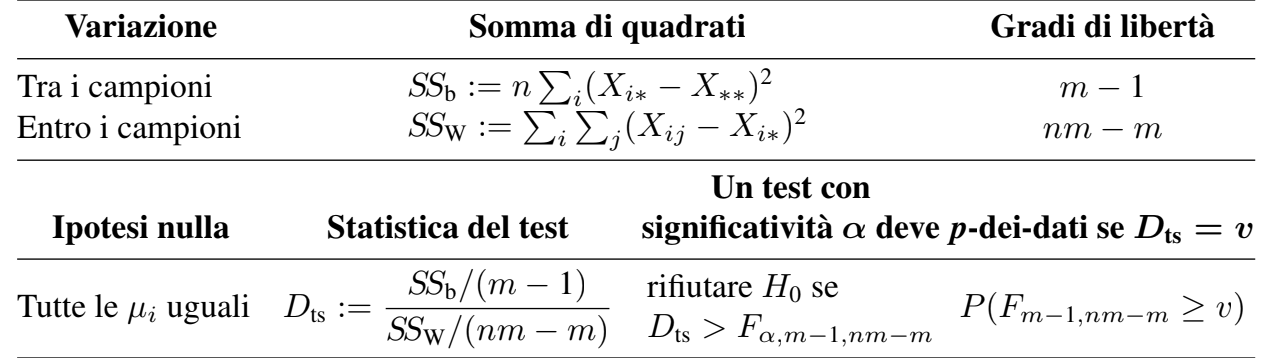
\includegraphics[width=\textwidth]{images/boh_11.png}
    \end{figure}
    \section{Regressione lineare}
    Molti problemi di statistica prevedono una singola variabile $Y$ di \emph{risposta} e un certo numero di variabili $\boldsymbol{x_1, x_2, \ldots, x_r}$ di \emph{ingresso}. La \emph{risposta} è in funzione dei dati, $Y$ è anche detta \emph{variabile dipendente}, mentre le $x_i$ sono le \emph{variabili indipendenti}.\\
    La più semplice relazione potrebbe essere quella lineare:
    \[ Y = \beta_0 + \beta_1x_1 + \ldots  + \beta_rx_r \]
    \centerline{Dove $\beta_0, \beta_1, \ldots, \beta_r$ sono costanti.} \\[2ex]
    Predire esattamente le $\beta_i$ non è possibile, quindi all'equazione si aggiunge un \emph{errore casuale} denominato $e$:
    \[ Y = \beta_0 + \beta_1x_1 + \ldots + \beta_rx_r + e \]
    La variabile $e$ ha distribuzione normale standard. $e \sim \mathcal N(0,1)$ \\
    L'equazione qui sopra è chiamata \textbf{equazione di regressione lineare}. \\
    Questa esprime la regressione di \emph{Y} rispetto alle variabili indipendenti $x_1, x_2, \ldots, x_r$, mentre le costanti $\beta_0, \beta_1, \ldots, \beta_r$ sono dette \emph{coefficienti di regressione} e vanno normalmente stimate.
    Un equazione di regressione si dice \emph{semplice} se $r = 1$, e quindi c'è solo una variabile indipendente, negli altri casi si dice regressione \emph{multipla}.
    Quindi la relazione diventa:
    \[ Y = \alpha + \beta x + e \]
    \subsection{Stima di parametri di regressione}
    Indichiamo con $A$ e $B$ (variabili aleatorie) degli stimatori di $\alpha, \beta$.
    L'equazione diventerà:
    \[ Y = A + Bx + e \]
    Per avvicinarsi alla retta reale la quantità $\boldsymbol{(Y_i - A + Bx_i)^2}$ deve risultare minima.
    (rappresenta il quadrato della differenza tra predizione e valore osservato)
    Quindi:
    \[ SS := \sum_{i = 1}^{n}(Y_i-A-Bx_i)^2 \]
    \centerline{Somma dei quadrati degli scarti tra risposte \textit{stimate} e \textit{reali}}
    \subsubsection{Metodo dei minimi quadrati}
    Ricaviamo $A$ e $B$ tale per cui la $SS$ risulta minima:
    \begin{equation*}
        \begin{split}
            &A = \overline Y - B \overline x \\
            &B = \frac{\sum_ix_iY_i - \overline{x}\sum_i Y_i }{\sum_i x_i^2 - n \overline x^2}
        \end{split}
    \end{equation*}
    La retta $Y = A + Bx + e$ è \emph{la stima della retta di regressione}.   
    \section{Distribuzione degli stimatori}
    $Y_1, Y_2, \ldots, Y_n$ sono indipendenti con distribuzione normale. $Y_i \sim \mathcal N(\alpha + \beta x_i, \sigma^2)$
    $B$ e $A$ anch'esse hanno distribuzione normale.
    $B$ è uno stimatore non distorto di $\beta$ perché il suo valore atteso è uguale a $\beta$:
    \[ \ev{B} = \beta \]
    Quindi la sua varianza risulta essere:
    \[\text{Var}(B) = \frac{\sigma^2}{\sum_i x^2_i -n\overline x^2}\]
    Anche $A$ è uno stimatore non distorto di $\alpha$ perché il valore atteso è $\alpha$:
    \[  \ev{A} = \alpha \]
    Varianza di $A$:
    \[ \text{Var}(A) = \frac{\sigma^2 \sum_i x_i^2}{n(\sum_i x_i^2 - n \overline x^2)} \]
    Somma dei quadrati dei residui è usata per stimare la varianza degli errori, $\sigma^2$:
    \[ SS_R := \sum_i^n(Y_i - A - Bx_i)^2 \]
    La $SS_R$ ha distribuzione chi-quadro, con $n-2$ gradi di libertà:
    \[ \frac{SS_R}{\sigma^2} \sim \mathcal{X}^2_{n-2} \]
    Il valore atteso della $SS_R$ è uguale alla varianza, quindi è uno stimatore non distorto del parametro incognito $\sigma^2$:
    \[ \ev{\frac{SS_R}{\sigma^2}} = n - 2 \quad \Rightarrow \quad \ev{\frac{SS_R}{n-2}} = \sigma^2\] 
    \begin{equation*}
        \begin{split}
            &S_{xY} := \sum_{i=1}^n x_i Y_i - n \overline x \overline Y \quad \text{dispersione di $x$ e $Y$}\\
            &S_{xx} := \sum_{i = 1}^{n} x^2_i - n \overline x^2 \quad \text{dispersione di $x$ e $x$}\\
            &S_{YY} := \sum_{i=1}^{n} Y_i^2 - n \overline Y^2 \quad \text{dispersione di $Y$ e $Y$}
        \end{split}
    \end{equation*}
    Possiamo riscrivere B come:
    \[ B = \frac{\sum_ix_iY_i - \overline{x}\sum_i Y_i }{\sum_i x_i^2 - n \overline x^2} \quad \Rightarrow \quad B=\frac{S_{xY}}{S_{xx}}\]
    \paragraph{In generale:}
    Nel caso in cui $Y_i, i = 1,2,3,\ldots,n$  siano normali indipendenti con media $\alpha + \beta x_i$ e varianza $\sigma^2$, gli stimatori dei minimi quadrati per $\beta$ e $\alpha$ sono:
    \[ B = \frac{S_{xY}}{S_{xx}} \quad \quad A = \overline Y - B \overline x $$ e hanno distribuzione: $$ B \sim \mathcal N(\beta,\frac{\sigma^2}{S_{xx}}) \quad \quad A \sim \mathcal N(\alpha,\frac{\sigma^2 \sum_ix_i^2}{nS_{xx}}) \]
    La somma dei quadrati dei residui è calcolata tramite:
    \[ SS_R = \frac{S_{xx}S_{YY}- S_{xY}^2}{S_{xx}} \]
    La $SS_R$ ha distribuzione:
    \[ \frac{SS_R}{\sigma^2} \sim \mathcal X^2_{n-2} \]
    \section{Inferenza sui parametri della regressione}
    Quanto sono distanti $A$ e $B$ da $\alpha$ e $\beta$?
    Dobbiamo vedere l'intervallo di confidenza
    \subsection{Inferenza su $\beta$}
    Formula dell'intervallo di confidenza di $\beta$:
    \[ \beta \in B \pm \sqrt{\frac{SS_R}{(n-2)S_{xx}}} \sim t_{\frac{\alpha}{2}, n-2} \]
    Estesa:
    \[ P\Big(B - t_{\frac{\alpha}{2},n-2} \cdot \frac{\sqrt{SS_R}}{(n-2)S_{xx}} < \beta < B + t_{\frac{\alpha}{2},n-2} \cdot \frac{\sqrt{SS_R}}{(n-2)S_{xx}}\Big) \]
    \textbf{Importante}: $\alpha$ \textbf{NON} è il parametro della regressione, ma è il livello di confidenza.
    \subsection{Inferenza su $\alpha$}
    Formula dell'intervallo di confidenza di $\alpha$:
    \[ \alpha \in A \pm \frac{SS_R\sum_{i}{}x_i^2}{\sqrt{n(n-2)S_{xx}}} \sim t_{\frac{\alpha}{2},n-2} \]
    Dove la prima $\alpha$ è il coefficiente della retta mentre $\alpha$ nella t è il livello di confidenza.
    \subsection{Inferenza su $\alpha + \beta x_0$ (test su $\overline{Y}$)}
    Il valore atteso di $A + B x_0$ è uguale a $\alpha + \beta x_0$  quindi è uno stimatore non distorto:
    \[ \ev{A +B x_0} = \ev{A} + x_0 \ev{B} = \boldsymbol{\alpha + \beta x_0} \]
    La varianza è:
    \[ \text{Var}(A+Bx_0) = \sigma^2 \Big[\frac{1}{n} + \frac{(\overline x - x_0)^2}{S_{xx}}  \Big] \]
    qual'è la distribuzione di $A+Bx_0$?
    \[ A+Bx_0 \sim \mathcal N \Big(\alpha+\beta x_0, \sigma^2 \Big[ \frac{1}{n} + \frac{(\overline x - x_0)^2}{S_{xx}} \Big]\Big) \]
    \subsubsection{Intervalli di confidenza}
    intervallo di confidenza di $\alpha + \beta x_0$:
    \[ \alpha + \beta x_0 \in A + B x_0 \pm t_{\frac{\alpha}{n}, n-2}\sqrt{\frac{1}{n} + \frac{(x_0- \overline x)^2}{S_{xx}}} \cdot \sqrt{\Big(\frac{SS_R}{n-2} \Big)} \]
    \centerline{$S_{xx}$ risulta piccolo se i punti sono vicini alla media.}
    \newpage
    \subsection{Inferenza di $Y_0 = Y(x_0) \rightarrow$ predittivo}
    Nel caso dovessimo prevedere un nuovo elemento della retta di regressione (utilizzando i dati già a disposizione) dobbiamo utilizzare la seguente formula:
    \[ A+Bx_0 \pm t_{\frac{\alpha}{2},n-2} \cdot \sqrt{\Big(1+\frac{1}{n} + \frac{(x_0-\overline x)^2}{S_{xx}}\Big)\frac{SS_R}{n-2}} \]
    \paragraph{Riassunto} Delle distribuzioni
    \begin{figure}[H]
        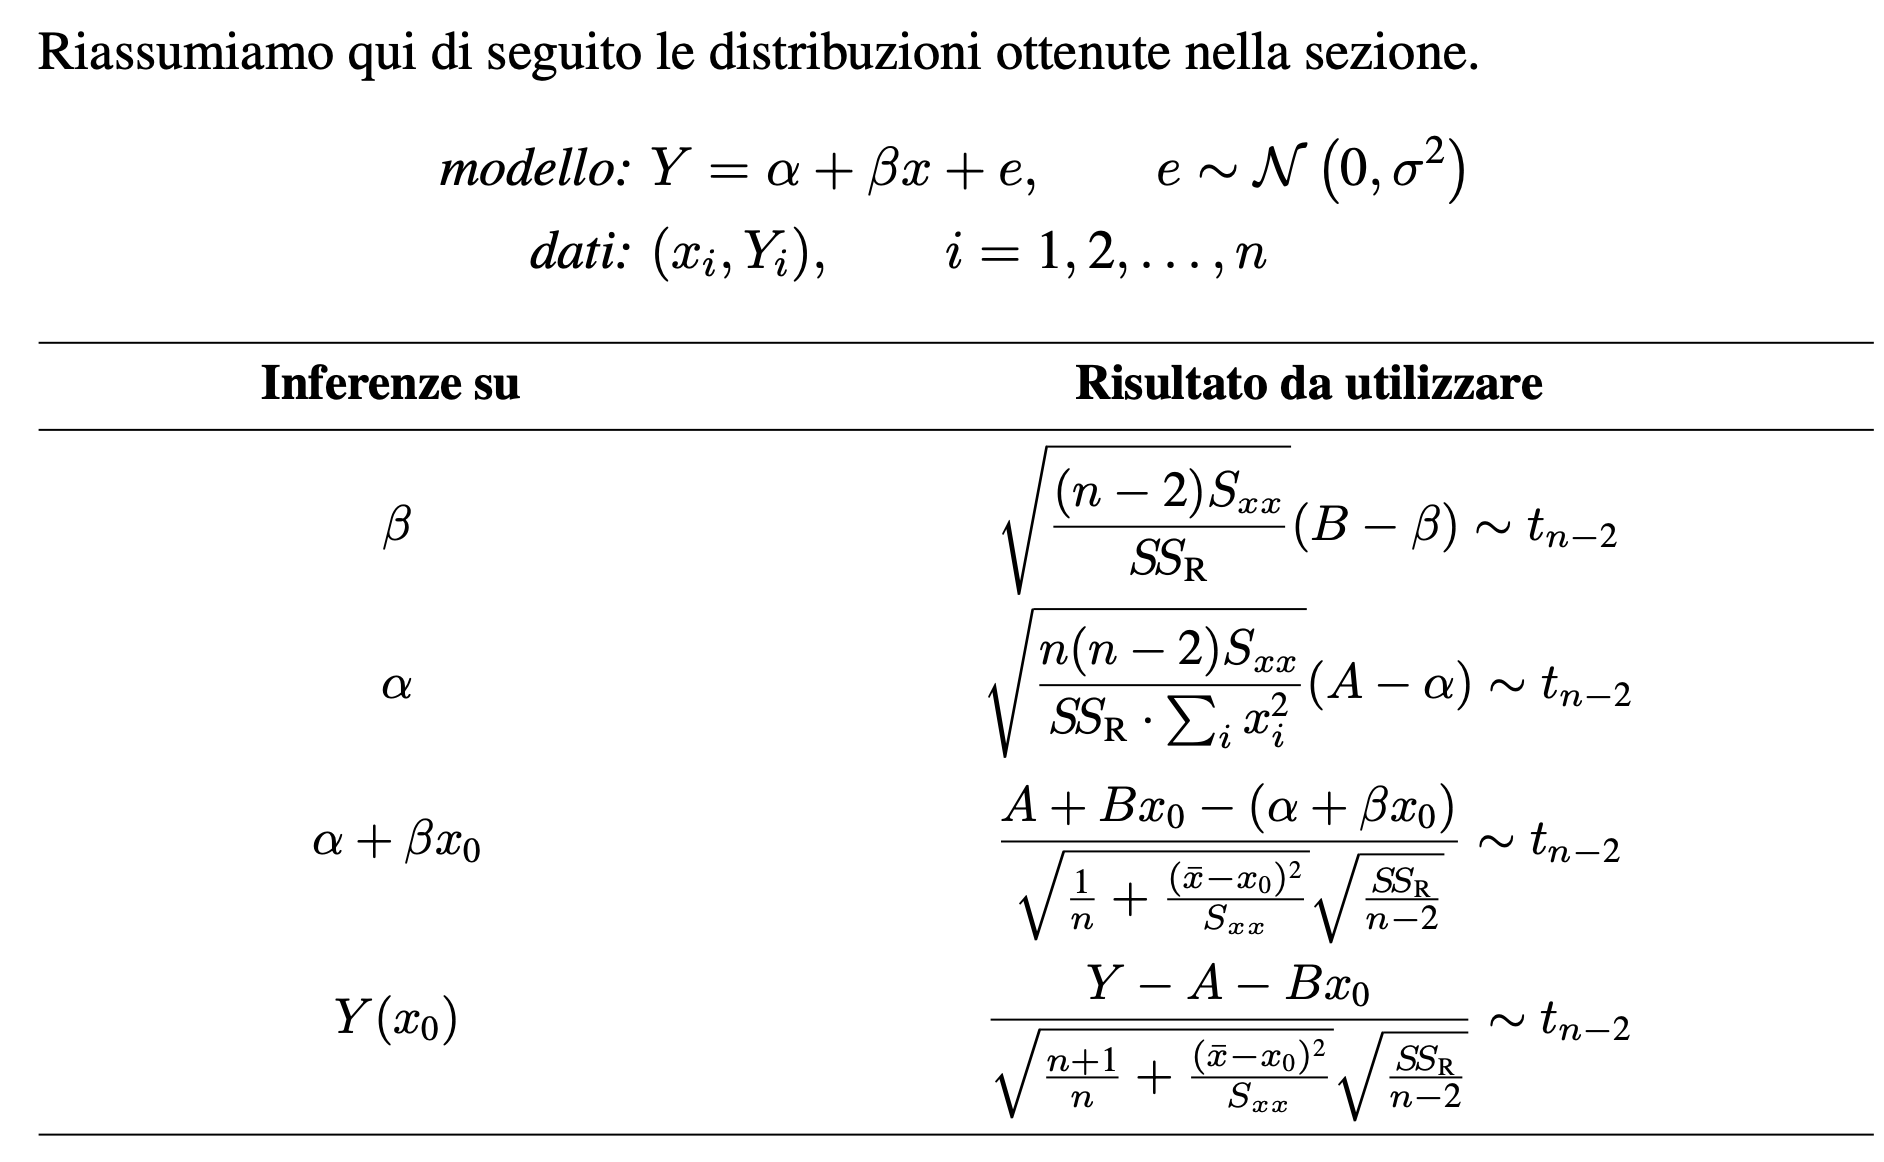
\includegraphics[width=\textwidth]{images/boh_13.png}
    \end{figure}
    \subsection{Coefficiente di determinazione}
    Come verifico i miei valori (della retta)? Tramite il \textit{coefficiente di determinazione.}
    Formula del coefficiente di determinazione:
    \[ R^2 = \frac{S_{YY}-SS_R}{S_{YY}} = 1- \frac{SS_R}{S_{YY}} \quad  \quad 0 \leq R^2 \leq 1 \]
    Casi possibili:
    \begin{enumerate}
        \item Se $R^2 = 1$:
        \begin{enumerate}
            \item la dispersione è data solo dalla retta (regressione)
        \end{enumerate}
        \item Se $R^2 = 0$:
        \begin{enumerate}
            \item la dispersione è dovuta solo dal rumore
        \end{enumerate}
    \end{enumerate}
    \textbf{La retta è migliore più $\boldsymbol{R^2}$ è vicino a 1}.
    \begin{figure}[H]
        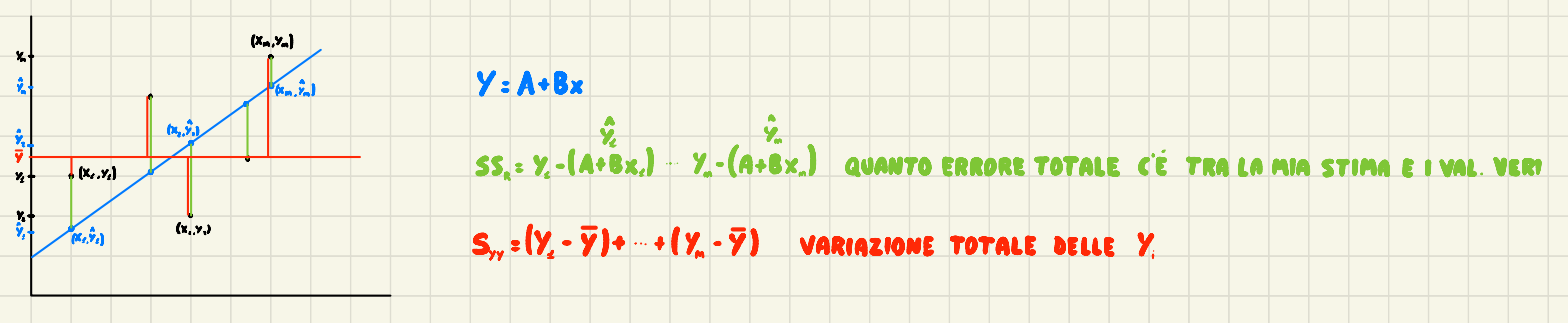
\includegraphics[width=\textwidth]{images/boh_14.png}
    \end{figure}
    \subsection{Coefficiente di correlazione}
    \[ r = \frac{\sum_i (x_i - \overline x)(y_i - \overline y)}{\sqrt{\sum_i (x_i - \overline x)^2 \sum_i(y_i - \overline y)^2}} = \frac{S_{xY}}{\sqrt{S_{xx}S_{YY}}} \]
    Dimostrazione matematica di $R^2$:
    \[ r^2 = \frac{S_{xY}^2}{S_{xx}S_{YY}} = \ldots = \boldsymbol{1- \frac{SS_R}{S_{YY}}} \]
    Quindi:
    \[ \boldsymbol{|r| = \sqrt{R^2}} \]
    \subsection{Analisi dei residui}
    Se il nostro modello non segue la forma di una "retta" non possiamo utilizzare la retta di regressione per rappresentare i nostri dati.
    \subsection{Trasformazione al lineare}
    Si può linearizzare tramite diverse funzioni, quella esponenziale in questo modo:
    \[ W(t) = ce^{-dt}\]
    \centerline{dove $e, t$ sono parametri} \\[2ex]
    Calcoliamo il log:
    \[ \log({W}(t)) \approx \log{(c)}-dt \]
    Se ora poniamo:
    \begin{itemize}
        \item $Y = \log{W(t)}$
        \item $\alpha = \log{c}$
        \item $\beta = -d$
    \end{itemize}
    La regressione lineare:
    \[ Y = \alpha + \beta t + e \quad \text{ diventa } \quad W(t) \approx e^{A+Bt} \]
    \subsection{Rimedio al caso eteroschedastico}
    Nel modello eterschedastico la varianza è in funzione della $x$. \\
    Ovvero l'errore cresce in base alle $x$. \\[2ex]
    Formula della \textit{varianza degli errori}:
    \[ \text{Var}(e_i)=\frac{\sigma^2}{W_i} \]
    La $W_i$ è il peso nel caso eteroschedastico:
    \[ W_i=\frac{1}{x_i} \]
    Formula della somma dei quadrati dei residui moltiplicato per il peso:
    \[ \sum_iW_i(Y-(A+Bx_0))^2 \]
    \subsection{Regressione lineare multipla}
    \[ Y = \beta_0 + \beta_1 x_1 + \beta_2 x_2 \ldots + \beta_k x_k +e \]
    \[ \min\sum_i(Y_i -(\beta_0+\beta_1x_{i1} + \beta_2x_{i2} \ldots + \beta_kx_{ik})) \]
    \subsection{Regressione (lineare) polinomiali}
    Nel caso in cui il nostro modello non può essere approssimato con un modelli lineari, si possono utilizzare relazioni polinomiali:
    \[ Y = \beta_0 + \beta_1x+\beta_2x^2 +\ldots+\beta_kx^k + e \]
    Dobbiamo minimizzare:
    \[ \sum_i^n (Y_i-B_0-B_1x_1-\ldots-B_rx_i^r)^2 \]
    Per determinare $\beta_0, \beta_1, \ldots, \beta_r$ dobbiamo
    \section{Stima di affidabilità dei sistemi}
    \subsection{Introduzione}
    In questa sezione prendiamo in considerazione una popolazione di oggetti i cui tempi di vita sono \textit{variabili aleatorie} con distribuzione comune. \\
    L'obiettivo di questo capitolo è quello di usare tutti i dati che abbiamo per stimare \textbf{un parametro incognito} \\
    Nella sezione \textit{14.2} viene introdotto il concetto di \textit{funzione di rischio (o intensità di rotture)}, mentre nella sezione \textit{14.3} ci concentriamo sulla \textit{legge esponenziale}
    \subsection{Funzione di intensità di rotture}
    Consideriamo una var. aleatoria $X$ \textit{continua e positiva}, e rappresenta il tempo di vita di un certo tipo di oggetti. \\
    Se abbiamo come $F$ la \textit{funzione di ripartizione} e $f$ la \textit{densità di probabilità} \\
    La sua \textbf{funzione di rischio / intensità di rotture} è la funzione $\lambda$ definita da:
    \[ \lambda(t) := \frac{f(t)}{1 - F(t)} \]
    Noi vogliamo studiare un elemento che è soggetto a \textit{rotture}, che funziona \textit{ininterrotamente} da un tempo $t$ \\
    Quindi noi vogliamo cercare una probabilità condizionata, ossia la seguente:
    \begin{equation*}
        \begin{split}
            P(X \in (t, t+ dt) | X > t) &:= \frac{P(X \in (t,t+dt), X > t)}{P(X>t)} \\
            &= \frac{P(X \in (t,t+dt))}{1 -F(t)} \\
            &\approx \frac{f(t) dt}{1-F(t)} =: \boldsymbol{\lambda(t) dt}
        \end{split}
    \end{equation*}
    In questo caso quindi $\lambda(t)$ rappresenta la densità condizionale di probabilità, che un oggetti si guasti nel prossimo istante
    \paragraph{In caso di distribuzione esponenziale} In questo caso la distribuzione della vita residua di un oggetto di eta $t$ è identica a quella di un oggetto nuovo, quindi dobbiamo avere un \textbf{valore costante}:
    \[ \lambda(t) := \frac{\lambda e^{-\lambda t}}{e^{-\lambda t}} = \boldsymbol{\lambda} \]
    \centerline{Il valore trovato è \textit{l'intensità della distribuzione esponenziale}} \\[2ex]
    La funzione $\lambda$ determina \textbf{univocamente} la $F$, quindi per definizione:
    \begin{equation}
        \begin{split}
            \lambda(s) &:= \frac{f(s)}{1-F(s)} \\
            &= \frac{F'(s)}{1 - F(s)} \\
            &= \boldsymbol{- \frac{d}{ds} \log (1- F(s))}
        \end{split}
    \end{equation}
    Possiamo integrare sto mapazzone con i membri tra 0 e t ottenendo che:
    \[ \int_{0}^{t} \lambda(s) \, ds = - \log(1-F(t)) + \log (1-F(0)) = \boldsymbol{-\log (1-F(t))} \]
    Ottenendo alla fine che 
    \[ \boldsymbol{1 - F(t) = \exp \left\{ - \int_{0}^{t} \lambda(s) \, ds \right\}} \]
    La funzione di ripartizione di una var. aleatoria continua può essere specificata tramite la \textit{corrispondente funzione di intensità di rotture}
    \subsection{Il ruolo della distribuzione esponenziale}
    \subsubsection{Interruzione al fallimento r-esimo}
    in questa sezione vediamo l'esame simultaneo di un campione di $n$ oggetti con \textit{tempi di vita esponenziali} e \textit{indipendenti} con media incognita $\theta$ e terminiamo il test non appena raggiungiamo un numero fissato $r \leq n$ \\
    I dati che abbiamo sono gli \textit{r} tempi di vita registrati, nel seguente ordine:
    \[ x_1 \leq x_2 \leq \cdots \leq x_r \]
    Se denotiamo con $X_i$ il tempo di vita dell'oggetto possiamo riassumere la parte di sopra come segue:
    \[ X_{i1} = x_1, X_{i2} = x_2, \ldots, X_{ir} = x_r \]
    La \textit{densità di probabilità} delle $X_{ij}$ è
    \[ f_{X_{i_j}} (x_j) = \frac{1}{\theta} e^{-x_j / \theta}, \qquad j = 1,2,\ldots, r \]
    La \textit{densità congiunta} invece è la seguente:
    \[ f_{X_{i_j}, \ldots, X_{i_r}} (x_1, \ldots, x_r) = \prod_{j=1}^{r} \frac{1}{\theta} e^{x_j / \theta} \]
    Per verificare la probabilità che le altre $n-r$ siano tutte maggiori $x_r$ è data dall'indipendenza:
    \[ P(X_j > x_r \text{ per } j \not = \{ i_1, i_2, \ldots, i_r \}) = (e^{-x_r / \theta})^{n-r} \]
    \begin{figure}[H]
        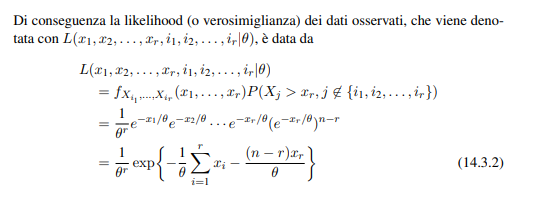
\includegraphics[width=\textwidth]{images/boh_12.png}
    \end{figure}
    Se abbiamo bisogno della verosomiglianza in \textit{funzione} solo degli $r$ tempi di rottura, la funzione di likelihood sarebbe:
    \[ f(x_1, x_2, \ldots, x_r) = \frac{n!}{(n-r)! \theta^r} \exp \left\{ \frac{1}{\theta} \sum_{i=1}^{r} x_i - \frac{(n-r) x_r}{\theta} \right\} \]
    Per calcolare lo stimatore di massima verosomiglianza di $\theta$ invece facciamo cosi:
    \[ \hat{\theta} := \frac{\sum_{i=1}^{r} X_{(i)} + (n-r) X_{(r)}}{r} =: \frac{\tau}{r} \]
    \centerline{Dove $\tau$ viene definito come \textbf{Total Time of Test statistic}} \\[2ex]
    $\tau$ rappresenta la somma delle statistiche $Y_i$ per $i=1,2,\ldots,r$ che indicano il tempo totale di funzionamento racchiuso tra la rottura dell'oggetti (i-1)-esimo e quella dell'i-esimo \\
    Il calcolo per trovarlo è il seguente 
    \[ \tau = \frac{j=1}{r} Y_j \]
    Dato che la \textit{somma} di variabili aleatorie esponenziali ha distribuzione \textit{gamma} otteniamo che il nostro $\tau$ è una \textbf{gamma} con parametri $r$ e $1 / \theta$ \\
    Sfruttando questa relazione:
    \[ \frac{2 \tau}{\theta} \sim \mathcal{X}^2_{2r} \]
    Notiamo subito (ensomma) che:
    \[ P(\mathcal{X}^2_{1-\frac{\alpha}{2}, 2r} < 2 \tau / \theta < \mathcal{X}^2_{1\frac{\alpha}{2}, 2r}) = \boldsymbol{1 -\alpha} \]
    E quindi sappiamo che abbiamo un livello di confidenza $\boldsymbol{1- \alpha}$ nell'affermare che:
    \[ \theta \in \left( \frac{2 \tau}{\mathcal{X}^2_{\frac{\alpha}{2}, 2r}}, \quad \frac{2\tau}{\mathcal{X}^2_{1- \frac{\alpha}{2}, 2r}} \right) \]
    \centerline{Questo per il caso \textbf{bilaterale}}
    \paragraph{Esempio} 50 transistor vengono messi in funzione simultaneamente. L'esperimento si conclude quando il 15-esimo ($r$) si rompe.
    Il Total time on test è di 525 ore ($TTT$). Trovare un intervallo di confidenza del 95\% per la vita media di un componente.
    La distribuzione è esponenziale. \\
    Mediamente si rompono:
    \begin{equation*}
        \begin{split}
            &\hat \theta = \frac{TTT}{r} \qquad \text{numero medio di guasti in 525 ore} \\
            &\hat \theta = \frac{525}{15} = 35
        \end{split}
    \end{equation*}
    Per trovare il livello di confidenza (dio merda) utilizziamo:
    \begin{equation*}
        \begin{split}
            &\theta \in \Big(\frac{2TTT}{\mathcal{X}^2_{\frac{\alpha}{2},2r}},\frac{2TTT}{\mathcal{X}^2_{1-\frac{\alpha}{2},2r}}   \Big) \\[2ex]
            &\boldsymbol{\theta \approx (22.35, 62.54)}
        \end{split}
    \end{equation*}
    \subsection{prove simultanee}
    Dobbiamo analizzare una sequenza una serie di oggetti, ciascuno e tempo di vita esponenziale con media sconosciuta $\theta$. L'esperimento viene concluso dopo un periodo prefissato $T$.
    I dati che abbiamo sono il numero $r$ di oggetti guasti entro $T$ e il tempo di vita di ogni oggetto $x_1,x_2, \ldots_, x_r$.
    \paragraph{MLE della media}: numero medio di oggetti che si rompono fino a $T$:
    $$\hat{\theta} = \frac{T}{r}$$
    \paragraph{Intervallo di confidenza di $\hat{\theta}$}:
    $$ \theta \in \Big( \frac{2T}{\mathcal X_{1-\frac{\alpha}{2},2r}^2}, \frac{2T}{\mathcal X_{\frac{\alpha}{2}},2r}^2  \Big) $$
\end{document}